%%%%%%%%%%%%%%%%%%%%%%%%%%%%%%%%%%%%%%%%%%%%%%%%%%%%%%%%%%%%%%%%%%%%%%%%%%%
%
% Plantilla para informe de práctica, DISC, UCN.
% Original por Felipe Narváez, versión modificada por Brian Keith.
% Compilar dos veces, por razones de que el compilador crea un archivo 
% para la tabla de contenido, para que este funcione compilar una vez más.
%
%%%%%%%%%%%%%%%%%%%%%%%%%%%%%%%%%%%%%%%%%%%%%%%%%%%%%%%%%%%%%%%%%%%%%%%%%%%
\documentclass[oneside,12pt, letterpaper, titlepage]{book}
% Esto es para poder escribir acentos directamente:
\usepackage[utf8x]{inputenc}
% Esto es para que el LaTeX sepa que el texto esta en español:
\usepackage[spanish,activeacute,es-lcroman]{babel}
% Paquetes de la AMS:
\usepackage{amsmath, amsthm, amsfonts}
%Otros paquetes necesarios.
\usepackage{graphicx}
\usepackage[tc]{titlepic}
\usepackage{fancyhdr}
\usepackage[T1]{fontenc}
\usepackage{titlesec}
\usepackage{float}
\usepackage{pslatex}  %Esto utiliza la fuente Times Roman (Casi indistinguible de Times New Roman)
\usepackage[titletoc]{appendix} %Este paquete para los anexos.
\usepackage{setspace} %Para espacio de 1.5
\usepackage{listings} %Código C#
\usepackage{multirow} %Tablas con fusiones de fila.
\usepackage{rotating}
\usepackage[numbers]{natbib}
\usepackage[nounderscore]{syntax}

\usepackage[none]{hyphenat} % Evita que las palabras sean cortadas

%\usepackage{tocloft}
%\renewcommand\cftchapnumwidth{10em}
%--------------------------------------------------------------------------
% Defino un nuevo comando para agregar espacios de 20 puntos, para utilizar
% 20 espacios solo utilizar las palabras \hsp
\newcommand{\hsp}{\hspace{2pt}}
%--------------------------------------------------------------------------
% Defino el nuevo titulo para capítulos con números romanos, como por
% ejemplo:
% I Introducción.
\renewcommand{\thechapter}{\Roman{chapter}}
%--------------------------------------------------------------------------
% Defino el nuevo titulo para subsecciones de capítulos con números árabes
% como por ejemplo:
% 1.1 Antecedentes generales 
\renewcommand{\thesection}{\arabic{chapter}.\arabic{section}}
%--------------------------------------------------------------------------
\addto\captionsspanish{% Replace "english" with the language you use
  \renewcommand{\contentsname}%
    {Índice General}%
}
\renewcommand{\theequation}{\arabic{chapter}.\arabic{equation}}
%--------------------------------------------------------------------------
% Defino el nuevo titulo para figuras de capitulos con numeros arabes
% como por ejemplo:
% 1.1 Antecedentes generales 
\renewcommand{\thefigure}{\arabic{chapter}.\arabic{figure}}
%--------------------------------------------------------------------------
\renewcommand{\thetable}{\arabic{chapter}.\arabic{table}}
%--------------------------------------------------------------------------
\titleformat*{\section}{\fontsize{12}{12}\bfseries}
\titleformat*{\subsection}{\fontsize{12}{12}\bfseries}
\titleformat*{\subsubsection}{\fontsize{12}{12}\bfseries}
%--------------------------------------------------------------------------
%Margenes de pagina.
\usepackage[top=2.5cm, bottom=2.5cm, left=2.5cm, right=2.5cm]{geometry}
%--------------------------------------------------------------------------
%Que aparezca la bibliografía en el índice.
%\usepackage{tocbibind}
%--------------------------------------------------------------------------
%Numeros de pagina en posiciones correctas.
\usepackage{fancyhdr} 
\pagestyle{myheadings}
\renewcommand{\headrulewidth}{0pt}
\fancyhead[L]{}
\fancyhead[R]{\nouppercase{\thepage}}
\fancyfoot[C]{}
%--------------------------------------------------------------------------
\usepackage{afterpage}
\usepackage{textcase}
\usepackage{enumitem}
%Listas ordenadas
\usepackage{datatool}
\newcommand{\sortitem}[1]{%
  \DTLnewrow{list}% Create a new entry
  \DTLnewdbentry{list}{description}{#1}% Add entry as description
}
\newenvironment{sortedlist}{%
  \DTLifdbexists{list}{\DTLcleardb{list}}{\DTLnewdb{list}}% Create new/discard old list
}{%
  \DTLsort{description}{list}% Sort list
  \begin{itemize}[leftmargin=*,label={}]%
    \DTLforeach*{list}{\theDesc=description}{%
      \item \theDesc}% Print each item
  \end{itemize}%
}
%Modificaciones a la tabla de contenidos.
\makeatletter    
\def\l@chapter{\@tocline{1}{0,2pt}{2pc}{8mm}{\ \ }} 
\def\numberSpaceChapter #1{#1.\enskip}% I added .\enskip because without these the dots and the space between the number and the title would disappear altogether.

%Esto se encarga que los capítulos tengan puntos en su tab leader.
\renewcommand*\l@chapter[2]{%
  \ifnum \c@tocdepth >\m@ne
    \addpenalty{-\@highpenalty}%
    \vskip 1.0em \@plus\p@
    \setlength\@tempdima{1.5em}%
    \begingroup
      \parindent \z@ \rightskip \@pnumwidth
      \parfillskip -\@pnumwidth
      \leavevmode \bfseries
      \advance\leftskip\@tempdima
      \hskip -\leftskip 
      \@pnum@font #1\nobreak
      \xleaders\hbox{$\m@th
        \mkern \@dotsep mu\hbox{.}\mkern \@dotsep
        mu$}\hfill%
      \nobreak\hb@xt@\@pnumwidth{\hss\@pnum@font #2}\par
      \penalty\@highpenalty
      %Esto le quita la negrita.
    \endgroup
  \fi}
%Esto renueva los comandos asociados a los otros elementos de la tabla de contenidos para que todo quede bien.
\renewcommand*\l@section{\@dottedtocline{1}{1.5em}{2.3em}}
\renewcommand*\l@subsection{\@dottedtocline{2}{3.8em}{3.2em}}
\renewcommand*\l@subsubsection{\@dottedtocline{3}{7.0em}{4.1em}}
\renewcommand*\l@paragraph{\@dottedtocline{4}{10em}{5em}}
\renewcommand*\l@subparagraph{\@dottedtocline{5}{12em}{6em}}
%Esto se encarga de quitarle la negrita a la frontmatter.
\g@addto@macro{\frontmatter}{\addtocontents{toc}{\protect\def\protect\@pnum@font{\normalfont}}}
\g@addto@macro{\mainmatter}{\addtocontents{toc}{\protect\def\protect\@pnum@font{\bfseries}}}
\g@addto@macro{\backmatter}{\addtocontents{toc}{\protect\def\protect\@pnum@font{\bfseries}}}
\makeatother
%--------------------------------------------------------------------------
% Comienza el documento
\begin{document}
\sloppy %Como \usepackage[none]{hyphenat} evita que las palabras se corten, esta línea realiza la corrección al texto justificado.
\renewcommand{\tablename}{Tabla}
\renewcommand{\listtablename}{Índice de Tablas}
\renewcommand{\listfigurename}{Índice de Figuras}
\setlength{\parindent}{0pt}

\onehalfspace

\begin{titlepage}
\centering
\vspace*{-0.4in}
%--------------------------------------------------------------------------
%Imagen o logotipo de la UCN

\includegraphics[scale=0.3]{./images/u.jpg}\\
{\fontsize{14}{14}\selectfont
UNIVERSIDAD CATÓLICA DEL NORTE\\
FACULTAD DE INGENIERÍA Y CIENCIAS GEOLÓGICAS\\
DEPARTAMENTO DE INGENIERÍA DE SISTEMAS Y COMPUTACIÓN\\}
\vspace{2.3in}
%--------------------------------------------------------------------------
% Titulo del documento
{\fontsize{14}{14}\bfseries Informe Práctica Pre Profesional\\}
%--------------------------------------------------------------------------
\vspace*{1.5in}
%--------------------------------------------------------------------------
%Datos Personales y/o profesores, alineados a la derecha de la hoja
\begin{flushleft}
\setlength{\leftskip}{7.2cm}
\fontsize{12}{12}\selectfont
{\setstretch{1.4}
Nombre Alumno: Nombre y Apellido\\
Rut: 18.000.000-0\\
Carrera: Ingeniería Civil en Computación e Informática\\
Nivel: 11\\
Nombre Empresa: Ferrocarril de Antofagasta a Bolivia\\
Ciudad: Antofagasta\\
Fecha inicio: 02 de Enero del 2015\\
Fecha término: 27 de Febrero del 2015\\
}
\end{flushleft}

\vspace*{0.5in}
Antofagasta\\
Abril, 2015
\end{titlepage}

%--------------------------------------------------------------------------
\titleformat{\chapter}[hang]
{\fontsize{12}{12}\bfseries\centering}
{\Roman{chapter}{.}\hsp}{0pt}{\fontsize{12}{12}\bfseries}
\titlespacing{\chapter}{0cm}{-13.6pt}{0.21cm}[0cm]
%--------------------------------------------------------------------------
%Capitulos sin enumeracion, número de pagina en romano
\frontmatter
\setcounter{page}{2}
%--------------------------------------------------------------------------
% Esta es la TABLA DE CONTENIDO.
\tableofcontents
\addtocontents{toc}{\let\protect\numberline\protect\numberSpaceChapter}
\addtocontents{toc}{~\hfill\textbf{Página}\par}

%DESCOMENTAR LA LINEA SIGUIENTE SI ES QUE LA TABLA DE CONTENIDOS TIENE MAS DE UNA PAGINA.
\addtocontents{toc}{\protect\afterpage{~\hfill\textbf{Página}\par\medskip}}
\thispagestyle{plain}

%--------------------------------------------------------------------------
% Esta es la Tabla de Figuras
\listoffigures % Índice de figuras
\addtocontents{lof}{~\hfill\textbf{Página}\par}
\addcontentsline{toc}{chapter}{Índice de Figuras} % para que aparezca en la tabla de contenidos

%--------------------------------------------------------------------------
% Esta es el indice de Tablas
%\listoftables % indice de tablas
%\addtocontents{lot}{~\hfill\textbf{Página}\par}
%\addcontentsline{toc}{chapter}{Índice de Tablas} % para que aparezca en el indice de contenidos

\chapter{Nomenclatura}
\begin{sortedlist}
\sortitem{DTIC: Departamento de las Tecnologías de Información y Comunicaciones.}
\sortitem{DCSO: Departamento de las Continuidad y Seguridad Operacional.}
\sortitem{DPCT: Departamento de Programación y Control de Trenes.}
\sortitem{GOF: Gerencia de Operaciones Ferroviarias.}
\sortitem{TVL: Terminal de Vías Libre.}
\sortitem{FCAB: Ferrocarril de Antofagasta a Bolivia.}
\sortitem{GID: Gerencia de Innovación y Desarrollo.}
\sortitem{SGPCT: Sistema de Gestión, Programación y Control de Trenes.}
\sortitem{KPI: Key Performance Indicator.}
\sortitem{DPP: Desviación Promedio Porcentual.}
\sortitem{NCI: Nivel de Cumplimiento de Instrucciones.}
\sortitem{UCT: Unidad de Control.}
\sortitem{UPT: Unidad de Programación}
\sortitem{ERS: Especificación de Requerimientos de Sistema.}
\sortitem{CRR: Cantidad de Reprogramaciones Requeridas.}
\sortitem{CNP: Cantidad de No-Cumplimientos de Programación.}
\sortitem{SSxA: Servicios por Atender}
\end{sortedlist}

\newpage
\chapter{Glosario}
\begin{sortedlist}


    \sortitem{\textbf{Gramática de libre contexto:} Conocidas también como gramáticas de tipo 2 o gramáticas independientes
del contexto, son las que generan los lenguajes libres de contexto. Los lenguajes libres de contexto son aquellos que pueden ser reconocidos por un autómata de pila determinístico o no determinístico.}

    \sortitem{\textbf{Key performance indicator:}	Es una medida del nivel del desempeño de un proceso; el valor del indicador está directamente relacionado con un objetivo fijado de antemano. Normalmente se expresa en porcentajes.}
    
    \sortitem{\textbf{Lenguajes naturales controlados:} Son un subconjunto de los lenguajes naturales, obtenidos mediante la restricción de la gramática y vocabulario para reducir la ambigüedad y la complejidad. Existen dos tipos principales, aquellos que mejoran la legibilidad para humanos y los que permiten la automatización del análisis semántico.}
    
    \sortitem{\textbf{Observación in situ:} Técnica de obtención de requerimientos que se basa en la observación directa del modo de trabajo de los usuarios.}

    \sortitem{\textbf{Plan piloto:} Es un estudio de viabilidad, basado en un experimento de pequeña escala, que permite a una organización determinar como un proyecto de mayor escala funcionará en la práctica.}
    
    \sortitem{\textbf{Programa de trenes:} Corresponde al itinerario que deben cumplir los trenes con el objetivo de satisfacer los diferentes servicios por atender, en este contexto se define diariamente.}
    
    \sortitem{\textbf{Prototipo:} Versión incompleta del programa de software a desarrollar utilizado como método de validación y de pruebas.}
    
    \sortitem{\textbf{Stakeholders:} Son todas aquellas personas u organizaciones que afectan o son afectadas por el proyecto, ya sea de forma positiva o negativa.}
    
    \sortitem{\textbf{Workflow:} Consiste en un patrón orquestado de actividades de negocio repetibles, funciona utilizando sistemáticamente por una organización.}

\end{sortedlist}





\newpage
\chapter{Resumen}
El Departamento de Tecnologías de la Información y Comunicaciones (DTIC) del Ferrocarril de Antofagasta a Bolivia (FCAB), en el marco de constante mejora y apoyo a los procesos de las otras unidades de la empresa, propuso la realización de dos proyectos. Uno enmarcado en el contexto de la programación y control de los trenes, y el otro centrado en la mejora de la seguridad operacional dentro del desarrollo de las maniobras ferroviarias.
En el ámbito de los procesos de programación y control de trenes, se hace necesario realizar un levantamiento de requerimientos, y posterior análisis y diseño para la mejora del Sistema de Gestión, Programación y Control de Trenes (SGPCT) que entrega el soporte informático a dichos procesos. En lo referente a seguridad operacional, se contempla el levantamiento de los procesos de maniobras de trenes, con el objetivo de llevar un control adecuado del desarrollo de las maniobras ferroviarias, pues actualmente no existe un método para verificar el seguimiento de los protocolos de seguridad. El desarrollo de estos proyectos es muy importante para el FCAB, ya que permitirán mejorar los índices de productividad y seguridad operacional, respectivamente.


En primer lugar se realizó el levantamiento de requerimientos para el mejoramiento de los procesos asociados al SGPCT. Esta etapa presentó dificultades debido a la falta de claridad inicial de los stakeholders con respecto a sus propias necesidades. Los resultados se formalizaron en un documento de requerimientos que fue validado por los clientes. Posteriormente, el resto del tiempo dedicado a este proyecto consistió en análisis y diseño de las mejoras que se implementarían, con el fin de clarificar los requerimientos fue necesario el desarrollo de numerosos prototipos.

Para el modelamiento de las maniobras se debió realizar un estudio en terreno de los procedimientos de seguridad seguidos por los operadores y de la documentación existente. Luego, los expertos en seguridad operacional del ferrocarril validaron los modelos construidos. Posteriormente, se construyó un documento de análisis detallado y una propuesta con las consideraciones clave para el desarrollo del proyecto.

Además, se desarrolló una serie de otras actividades de apoyo al DTIC, específicamente un levantamiento de requerimientos para el área de servicios, la construcción de una planilla de indicadores, y la investigación de un algoritmo para la transferencia remota de archivos.

Los resultados más importantes de esta práctica corresponden al análisis y diseño de las mejoras para el SGPCT, que incluye un nuevo módulo de instrucciones para el programa de transporte de trenes que actualmente se trabaja en planillas electrónicas, y la definición de nuevos indicadores clave de rendimiento para medir la desviación de la ejecución con respecto a la programación y la calidad de ésta última. En el marco del levantamiento de los procesos de maniobras, se ha desarrollado una serie de modelos y propuestas que entregan las bases del proyecto, estos resultados fueron validados por los stakeholders, quienes finalmente aprobaron la continuación del proyecto por parte del DTIC.

%--------------------------------------------------------------------------
%Capitulos normales con enumeracion y con número de pagina arabes
\mainmatter
%--------------------------------------------------------------------------
% Defino el formato de titulo para el capitulo, numero romano y el titulo
% del capitulo separado con una linea de color gris, de esta forma:
% I | Introducción 
\titleformat{\chapter}[hang]
{\fontsize{12}{12}\bfseries}
{\Roman{chapter}{.}\hsp}{0pt}{\fontsize{12}{12}\bfseries}
\titlespacing{\chapter}{0cm}{-13.6pt}{0.21cm}[0cm]
%--------------------------------------------------------------------------
% TIP
% Para las secciones pueden probar como
% \section[nombre corto]{Nombre largo}
% El nombre corto aparecera en el indice de contenido
% el nombre largo aparecera como titulo de la sección
% Este tip tambien sirve para los chapters.
%--------------------------------------------------------------------------

\chapter[Introducción]{INTRODUCCIÓN}

\section{Descripción de la organización y departamento}

El Ferrocarril de Antofagasta a Bolivia (FCAB), parte del Grupo Antofagasta PLC, es una empresa con más de 120 años de trayectoria dedicados a brindar servicios de transporte en el norte de Chile. Se constituyó en Londres el año 1.888 cuando capitales ingleses adquirieron a la Compañía Huanchaca el ferrocarril y todos los derechos que dicha empresa mantenía en ese año. 

FCAB es hoy una empresa sólida y dinámica, que ha alcanzando un alto grado de desarrollo y que presta al cliente un servicio integral, brindando apoyo en la transferencia de carga, almacenamiento y el embarque, servicio combinado con camiones y apoyo informático. Esto es posible a través de instalaciones especializadas y personal altamente calificado, asegurando el mejor manejo de la carga.

Los servicios de FCAB a nivel regional, consisten primeramente del transporte de ácido sulfúrico y cátodos de cobre para las empresas mineras de la Región de Antofagasta. A nivel internacional, se destaca el transporte de plomo y concentrados de zinc desde Bolivia.

El FCAB tiene participación en la Empresa Ferroviaria Andina S.A., Antofagasta Terminal Internacional Ltda. e Inversiones Hornitos S.A. Además, es dueño del 100\% de las empresas Train Ltda., Ingeniería y Servicios Ltda., FCAB Ingeniería y Servicios Ltda. y  Aguas Antofagasta S.A.

La estructura organizativa del FCAB cuenta con ocho gerencias además de la gerencia general, como se puede observar en la figura \ref{fig:orgFCAB}.

\begin{figure}[H]
    \centering
    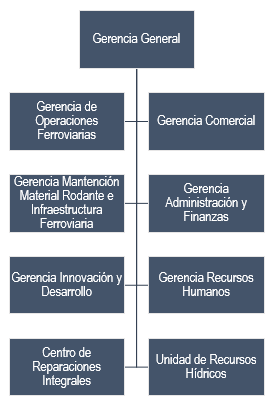
\includegraphics[scale=0.8]{./images/OrganigramaFCAB}
    \caption{Estructura organizacional del FCAB.}
    \label{fig:orgFCAB}
\end{figure}

FCAB es una empresa que busca la mejora continua de sus servicios, promoviendo la capacitación permanente de sus empleados y requiriendo la incorporación de nuevas tecnologías.

Como apoyo a estos procesos de mejora organizacional, el FCAB cuenta con la Gerencia de Innovación y Desarrollo (GID). La principal función de la GID dentro del FCAB es el desarrollo de nuevas tecnologías que entreguen un apoyo a las otras áreas y departamentos dentro de la organización. 

La GID está dividida en el Departamento de las Tecnologías de Información y Comunicaciones (DTIC) y el Departamento de Estudio. El DTIC está formado por ingenieros en computación e informático egresados de la Universidad Católica del Norte, y se divide en cuatro áreas: proyecto, soporte, estudio y telecomunicaciones. La estructura organizacional interna de la GID se puede observar en la figura \ref{fig:orgGID}.

\begin{figure}[H]
    \centering
    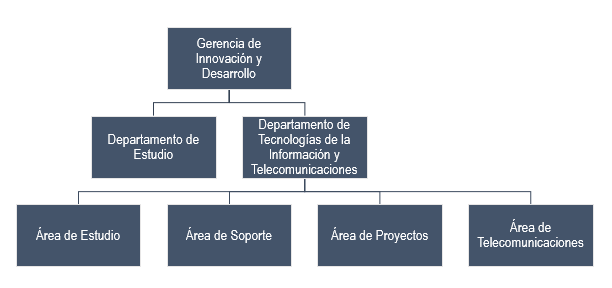
\includegraphics[scale=0.8]{./images/OrganigramaGID}
    \caption{Estructura organizacional interna de la GID.}
    \label{fig:orgGID}
\end{figure}

La informática actúa como una actividad de apoyo dentro de la organización, generando valor a través del desarrollo de  proyectos destinados a mejorar los procesos y el funcionamiento de las otras unidades empresariales. (Laudon y Laudon, 2004). De esta forma, el DTIC se posiciona entregando un apoyo transversal a todas las otras actividades de la empresa dentro de la cadena de valor, tanto a las primarias como a las de apoyo (Porter y Millar, 1985).

\section{Descripción general del trabajo realizado}
El trabajo realizado consistió en el desarrollo de dos proyectos, además de otros trabajos de menor longitud que se asignaron durante el periodo de práctica.

El primero de los proyectos consistía en la mejora del proceso de programación y control de trenes, mediante el análisis y diseño de un nuevo módulo para el SGPCT y el desarrollo de nuevos indicadores de rendimiento para el Departamento de Programación y Control de Trenes (DPCT). El objetivo de este trabajo es mejorar los procesos y los sistemas de apoyo del personal del DPCT. Este es el principal proyecto realizado durante el periodo de práctica y culminó con la entrega de un prototipo inicial y un manual de sistema con todas las especificaciones y análisis correspondientes. 

El segundo de los proyectos consistía en el levantamiento de los procesos de maniobras para los trenes de línea, esto con el fin de implementar un sistema en los equipos disponibles en cada locomotora, conocidos como Terminales de Vías Libres (TVL), que permitiese llevar un registro de los procedimientos de cada maniobra. El propósito de este registro es permitir a los supervisores del Departamento de Continuidad y Seguridad Operacional (DCSO) controlar de manera adecuada los procedimientos para mejorar el nivel de seguridad operacional. La primera fase del proyecto culminó con la entrega de un documento de análisis de procesos detallado junto con un resumen de las propuestas.

Entre las otras actividades contempladas se encuentra un levantamiento de requerimientos realizado para el área de servicios por petición del encargado de prácticas, el desarrollo y validación de una planilla de indicadores de rendimiento para el área de mantención, y finalmente, el análisis de un algoritmo de actualización remota para su uso en los TVL.

Para el proceso de toma de requerimientos se realizaron reuniones con los clientes y usuarios, además del uso de técnicas tales como la observación in situ y la revisión de documentos y protocolos. Los resultados de estos procesos fueron formalizados en documentos que luego fueron enviados para su validación a los clientes.

En el caso del proyecto de mejora del proceso de programación y control de trenes se desarrollaron prototipos con el fin de validar apropiadamente los requerimientos. Se debe notar también que los requerimientos emergentes que surgieron en cada reunión de avance fueron documentados y agregados a la especificación de requerimientos del sistema.

Todos los trabajos realizados fueron terminados en el tiempo correspondiente de acuerdo a la planificación, que fue realizada de tal forma de considerar suficiente holgura en caso de algún imprevisto. Se consideró fuera del alcance del periodo de práctica el traspaso del módulo de instrucciones y los reportes de los nuevos indicadores a los servidores de producción, quedando este trabajo pendiente para el periodo de marzo. 

\section{Lugar de trabajo}
Se asignó una oficina de tamaño medio compartida por todos los practicantes del DTIC. La oficina contaba con un computador de escritorio con Windows XP conectado a la intranet empresarial y con acceso a internet. 

Durante la práctica se contó con el apoyo del equipo del DTIC, incluyendo a los encargados de los sistemas del FCAB y del área de soporte, encargados de mantener en correcto funcionamiento todos los equipos y redes de la empresa. La distribución de las oficinas permitió una interacción constante con el encargado de práctica y los supervisores de los proyectos, facilitando así el trabajo a realizar.

Las reuniones de avance con el encargado de prácticas y los otros ingenieros informáticos supervisores se realizaron en la sala de reuniones de la GID. Las reuniones con los clientes se realizaron principalmente en la sala de reuniones de la Gerencia de Operaciones Ferroviarias (GOF) y en algunos casos en la misma GID. 

\section{Equipo de trabajo}
El equipo de trabajo consistió de dos personas, un practicante de Ingeniería Civil en Computación e Informática y un practica de Ingeniería Ejecución en Computación e Informática. El trabajo realizado se repartió de forma equitativa entre el equipo, aunque se procuró de hacerlo de tal forma de dar énfasis a los requerimientos propios de las prácticas profesionales de cada carrera.

El equipo fue supervisado por el encargado de prácticas del DTIC, quien actuó de guía durante el desarrollo de los proyectos. Además se contó con el apoyo del encargado del Sistema de Gestión, Programación y Control de Trenes (SGPCT), y en menor grado con el apoyo de los otros miembros del DTIC.

\section{Planificación del Trabajo}
Durante la primera semana, el encargado de práctica en conjunto con otros ingenieros del DTIC y los practicantes construyeron una versión inicial de la planificación. Además, se desarrolló una carta de proyecto donde se definían claramente los entregables y el alcance del proyecto.

Notar que originalmente no estaba contemplado el modelamiento de los procesos de maniobras en la planificación, pues este proyecto se inició a fines de enero. En la figura \ref{fig:Gantt} del anexo A se muestra una carta Gantt simplificada para ambos proyectos, esta versión no contempla las actividades de apoyo realizadas fuera del marco de los proyectos principales.



\chapter[Análisis y Diseño de Módulo de Instrucciones]{ANÁLISIS Y DISEÑO DE MÓDULO DE INSTRUCCIONES}
El propósito de este capítulo es explicar el trabajo realizado en el análisis y diseño del módulo de instrucciones para el programa de transporte de trenes.

\section{Descripción de la situación actual y problemática}
El FCAB cuenta con una serie de sistemas para apoyar el funcionamiento de las distintas gerencias y la operación diaria del negocio. El sistema de mayor criticidad en este ámbito es el SGPCT, pues toda la operación ferroviaria depende de éste, influyendo de este modo directamente sobre el funcionamiento de los servicios de la empresa.

El DPCT en conjunto con el DTIC se plantearon un proyecto de mejora del proceso de programación y control de trenes, y en consecuencia del SGPCT. El propósito del proyecto es transformar la programación en una herramienta de gestión. La primera etapa del proyecto contemplaba el análisis de los procesos actuales, y luego, en base a los resultados de esta primera etapa, se realizaría el diseño de las mejoras necesarias y finalmente la implementación de éstas. 

La principal motivación detrás de este proyecto es que actualmente existen ciertas etapas del proceso de programación y control que aún se realizan de forma manual, por lo que las jefaturas de la Unidad de Programación de Trenes (UPT) y la Unidad de Control de Trenes (UCT) se encontraban particularmente interesadas en automatizar estos procesos. Por otro lado, no se cuenta con indicadores que permitan determinar si la programación y el subsecuente control son adecuados, es por ello que se solicitó la definición indicadores para medir la calidad de la programación y la desviación real de la ejecución. 

\section{Objetivos}
En la primera reunión realizada al inicio de la práctica se determinaron los objetivos del proyecto. El objetivo general es la mejora del proceso de programación y control de trenes. Este proyecto permitirá optimizar los servicios de apoyo al personal de control y programación de trenes, lo que a su vez permitirá prestar un mejor servicio de transporte ferroviario. 

Entre los objetivos específicos determinados se contemplaron los siguientes.

\begin{itemize}
\item Automatizar el proceso de manejo de las instrucciones de los trenes.
\item Minimizar el tiempo consumido por los controladores en el manejo de instrucciones.
\item Integrar las interacciones con la lógica del SGPCT.
\item Definir indicadores clave de rendimiento (KPI) para el proceso de control de trenes.
\item Controlar la desviación del programa ejecutado con el programa original de trenes.
\end{itemize}

\section{Levantamiento de requerimientos}
El levantamiento inicial de requerimientos contempló un periodo de dos semanas en las cuáles se realizaron las siguientes actividades:

\begin{itemize}
\item Reuniones con los clientes.
\item Reuniones con los usuarios.
\item Observaciones in situ.
\item Capacitación sobre el módulo de programación del SGPCT.
\item Estudio y análisis de documentación oficial.
\item Entrevistas estructuradas y no estructuradas.

\end{itemize}

Estas actividades fueron desarrolladas múltiples veces con el fin de obtener una especificación de requerimientos completa y sin ambigüedades. Tal como indica Sommerville el proceso de toma de requerimientos fue iterativo y en cada vuelta del ciclo la comprensión por parte del equipo de trabajo fue mejorando (Sommerville, 2011). 

En las reuniones con los clientes se buscó entender el propósito del proyecto y los resultados esperados de las mejoras, además de la obtención de una perspectiva de alto nivel del funcionamiento de los procesos. En estas reuniones se encontró que la primera prioridad se le debía dar a la automatización del control de instrucciones del programa de transporte de trenes, que actualmente se controlaba de forma manual mediante una planilla electrónica y documentos impresos. La segunda prioridad era la definición de indicadores para medir la calidad de la programación y de la ejecución del programa, en términos de la desviación ocurrida en la operación.

En las reuniones con los usuarios (principalmente los controladores y asistentes de programación) se buscó obtener información sobre el detalle del funcionamiento actual de los procesos asociados al SGPCT, además de informales del proyecto que se estaba realizando, esto con el objetivo de incluirlos en el proceso de desarrollo y minimizar los efectos de la resistencia al cambio en cuánto se implementaran las mejoras.

Además de las reuniones se debieron realizar dos observaciones in situ en la sala de control, con el fin de entender la ejecución real del programa en el sistema por parte de los controladores de trenes y los administrativos.

También se dispuso de dos sesiones de capacitación con el asistente de programación, donde se explicó en detalle el funcionamiento del módulo de programación de trenes del SGPCT. En la primera sesión se explicó el funcionamiento general del módulo de programación, además de resolverse una serie de dudas sobre el funcionamiento actual del programa de transporte de trenes. En la segunda sesión se estudio el workflow completo de programación en el SGPCT.

También se dispuso de la documentación oficial del SGPCT, que a pesar de estar desactualizada permitió entender de mejor manera el sistema. Además de la documentación oficial, se encontraba disponible un levantamiento de proceso desarrollado por memoristas anteriores que habían estudiado los procesos del SGPCT, el documento entregado incluía los procesos de alto nivel asociados a todos los módulos del SGPCT, lamentablemente no se disponía de tantos detalles al nivel de precisión necesitado.

En base a los resultados obtenidos en estas primeras actividades se realizaron entrevistas estructuradas y no estructuradas con el fin de resolver las dudas pendientes con los usuarios y clientes. Estas entrevistas permitieron precisar de manera correcta los requerimientos obtenidos.

La información adquirida en todas estas actividades fue utilizada para construir el documento de especificación de requerimientos. Este documento fue evolucionando durante las primeras dos semanas y fue validado oficialmente al terminar este periodo por los principales stakeholders.

Se debe notar que uno de los problemas que se presentó fue definir claramente los resultados esperados por parte de los clientes y usuarios, ya que los stakeholders no tenían una claridad de lo que deseaban obtener y la falta de conocimiento del dominio dificultó inicialmente el proceso.

\section{Análisis}
En base al documento de Especificación de Requerimientos de Sistema (ERS) construido se procedió a analizar las mejoras que se deberían implementar. En el análisis se considero la infraestructura preexistente del SGPCT en conjunto con las nuevas necesidades y requerimientos detectados.

El análisis se centró en las instrucciones del programa de transporte de trenes, debido a que los clientes determinaron en las reuniones que esta era su primera prioridad. Posteriormente, se realizó la definición de los indicadores de rendimiento, utilizando como base los indicadores definidos en la planilla del programa de transporte de trenes y la bibliografía pertinente encontrada durante el desarrollo del análisis.

Se desarrollaron dos modelos referentes a los procesos de programación y control de instrucciones (ver figuras \ref{fig:MGP} y \ref{fig:MEI} en el anexo C respectivamente). La mejora del proceso abarca toda la etapa de control a cargo de la UCT y el desarrollo del programa de transporte de trenes por parte de la UPT.

Durante la fase de análisis se desarrollaron varios prototipos, éstos tienen como propósito ayudar en la obtención y validación de los requerimientos del sistema (Sommerville, 2011). Algunos prototipos fueron de uso interno para el equipo desarrollador y otros fueron mostrados a los clientes con el fin de verificar que los requerimientos se hayan entendido de manera adecuada.

\subsection{Lenguaje estructurado de instrucciones}
Se contempló el uso de un lenguaje semi-estructurado para la definición de instrucciones, de acuerdo a los éxitos presentados en otras industrias similares (Kuhn, 2013). Este lenguaje permitiría escribir instrucciones y luego compilarlas, este compilador de instrucciones generaría en base a la entrada todos los efectos necesarios sobre el SGPCT. No obstante, se consideró esta opción una mala alternativa de solución, principalmente debido a la complejidad inherente de las instrucciones, la dificultad de definición de un lenguaje adecuado y los problemas de mantenibilidad en que se incurriría al utilizar un compilador, debido a que los conocimientos necesarios para desarrollar y mantener un compilador son demasiado escasos.

A pesar de esto, se desarrolló un prototipo del compilador de instrucciones como prueba de concepto, esto incluyó la construcción de una gramática de libre contexto y de las especificaciones formales del lenguaje de instrucciones. El lenguaje creado abarca un 95\% de las instrucciones provistas por los clientes como ejemplos (el otro 5\% sería tratado excepcionalmente). El problema de este enfoque es que en la fase de análisis semántico se complicaría mucho la interpretación de la instrucción ingresada, no obstante la fase de análisis léxico y sintáctico fueron implementadas exitosamente en el prototipo de acuerdo al marco definido para la construcción de compiladores (Louden, 1997). La gramática de libre contexto construida se presenta en el anexo B.

\subsection{Clasificación de instrucciones}
A pesar del abandonó de la idea del lenguaje semi-estructurado para las instrucciones, el análisis realizado permitió definir de manera muy acotada los tipos de instrucciones y las dimensiones de estas que importaban.

Las instrucciones se clasificaron en dos tipos:
\begin{itemize}
\item Notificaciones: Aquellas instrucciones que deben ser recordadas pero no debe confirmarse su ejecución correcta o incorrecta (por ejemplo: "Recordar que a las 10.30 AM no hay comunicaciones'').
\item Alerta normal: Aquellas instrucciones que deben ser recordadas y debe además confirmarse su ejecución correcta o incorrecta (por ejemplo: "Tren 1201 recoge 13 carros en Mejillones'').
\item Alerta crítica: Aquellas instrucciones que por su nivel de criticidad deben ser realizadas correctamente y es necesario que se recuerden oportunamente. 
\end{itemize}

Además, se contemplaron las siguientes dimensiones asociadas a una instrucción:
\begin{itemize}
\item Tren: Las instrucciones pueden estar asociadas a trenes específicos.
\item Terminal: Las instrucciones pueden estar asociadas a terminales o estaciones específicas.
\item Horario: Las instrucciones pueden estar asociadas a un rango horario o a un horario puntual.
\end{itemize}

Esta clasificación fue posteriormente validada por el cliente, y fue el enfoque finalmente utilizado como base para la implementación del prototipo entregado.

\subsection{Formato de notificaciones y alertas}
Una vez definidas las instrucciones a nivel de programación fue necesario determinar en qué formato y de qué manera se mostrarían a los controladores durante la ejecución del programa de transporte de trenes. Debido a la importancia de que los controladores atiendan estas notificaciones y alertas, era necesario definir esto de forma apropiada.

Se contemplaron diversas alternativas, con grados de complejidad variables desde una simple ventana de alertas en el navegador hasta el uso de librerías más complejas en Javascript que utilizaran animaciones más complejas para llamar la atención del controlador. Se debió decidir también si las alertas serían restrictivas o permitirían al usuario seguir utilizando el sistema aún sin atender la instrucción. 

Finalmente se optó por el uso de una nueva interfaz que se mostraría en un pop-up al controlador y le impediría al usuario realizar cualquier otra acción hasta atender la instrucción. Originalmente no se contemplaba usar un enfoque restrictivo, sin embargo, los clientes solicitaron el uso de esta modalidad.

\subsection{Definición de los indicadores de rendimiento}
Se definieron cuatro KPI’s, bajo los criterios de medir calidad, desviación y cumplimiento. Los indicadores se basaron en el trabajo realizado por Schittenhelm y Landex para medir el rendimiento de las tablas de programación ferroviarias (Schittenhelm y Landex, 2012) y en la información entregada por los clientes.

\begin{itemize}
\item Desviación Porcentual Promedio (DPP): Mide la desviación porcentual promedio por cada tren del tiempo de ejecución con respecto al tiempo programado. Esto se realiza con respecto a la programación original del día, no se calcula con respecto a reprogramaciones.
\item Cantidad de Reprogramaciones Requeridas (CRR): Mide cuantas veces fue necesario reprogramar durante el transcurso de la ejecución.
\item Nivel de Cumplimiento de Instrucciones (NCI): Mide el porcentaje de cumplimiento de la programación asociado a las instrucciones del día.
\item Cantidad de No-Cumplimientos de Programación (CNP): Mide cuantos eventos programados no se han cumplido con respecto a la programación. Este valor es diferente para cada reprogramación.
\end{itemize}

Para validar la utilidad de estos indicadores se incluyeron en el desarrollo del prototipo que se entregaría al final de la práctica. No obstante, debido a que el tiempo destinado a la construcción del prototipo era limitado, se optó por implementar los dos más importantes, correspondientes a la DPP y al NCI. El prototipo entregado genera un reporte con estos indicadores, además de entregar el detalle de los datos utilizados para los cálculos. Los reportes están destinados al jefe del DPCT, el jefe de la UCT y el jefe de la UPT según se define en cada caso.

La DPP se consideró importante ya que encajaba dentro de los objetivos indicados por el cliente, en específico con medir la desviación de la ejecución real y la calidad del programa de trenes. Este indicador se define como el promedio de los desvíos porcentuales entre el tiempo de programación y el tiempo de ejecución por cada tren  (en términos absolutos, pues en caso que un tren se adelante la diferencia sería negativa). Se define mediante la siguiente fórmula:

\begin{equation}
DPP = \sum_{t \in trenes}
{\left | {\frac{TE_{t}-TP_{t}}{TP_{t}}} \right |} \cdot \frac{100}{n}
\end{equation}

Donde se define $TE_{t}$ como el tiempo de viaje ejecutado en que el tren llegó al terminal de destino, $TP_{t}$ como el tiempo de viaje programado en que el tren debería llegar al terminal de destino, y $n$ como la cantidad de trenes diarios. 

Por otra parte, el NCI se consideró importante por encontrarse definido en la planilla de instrucciones original entregada por la UPT. En base a las definiciones entregadas se utilizó la siguiente fórmula:

\begin{equation}
NCI = \Bigg\{ \begin{matrix} 
 0, & TI-NE-NS = 0  
\\
 \frac{IC}{TI-NO-NS}, & d.o.m. 
 \end{matrix}
\end{equation}

Donde $TI$ es el total de instrucciones diarias, $NE$ es la cantidad de instrucciones no cumplidas debido a una falla de ejecución, $NS$ es la cantidad de instrucciones no cumplidas debido a suspensión, e $IC$ es la cantidad de instrucciones cumplidas. Esta fórmula está basada en los indicadores definidos en la planilla original utilizada por la UPT y fue validada por los clientes.

\section{Solución propuesta}
La solución propuesta contempla la incorporación de un nuevo módulo al SGPCT. El nuevo módulo debe interactuar en todo momento con el SGPCT y además requiere obtener información de las mismas fuentes de datos. 

En la figura \ref{fig:diagramaPTT} se resumen los principales submódulos del sistema con el objetivo de proveer una visión de alto nivel del sistema diseñado. 

\begin{figure}[H]
    \centering
    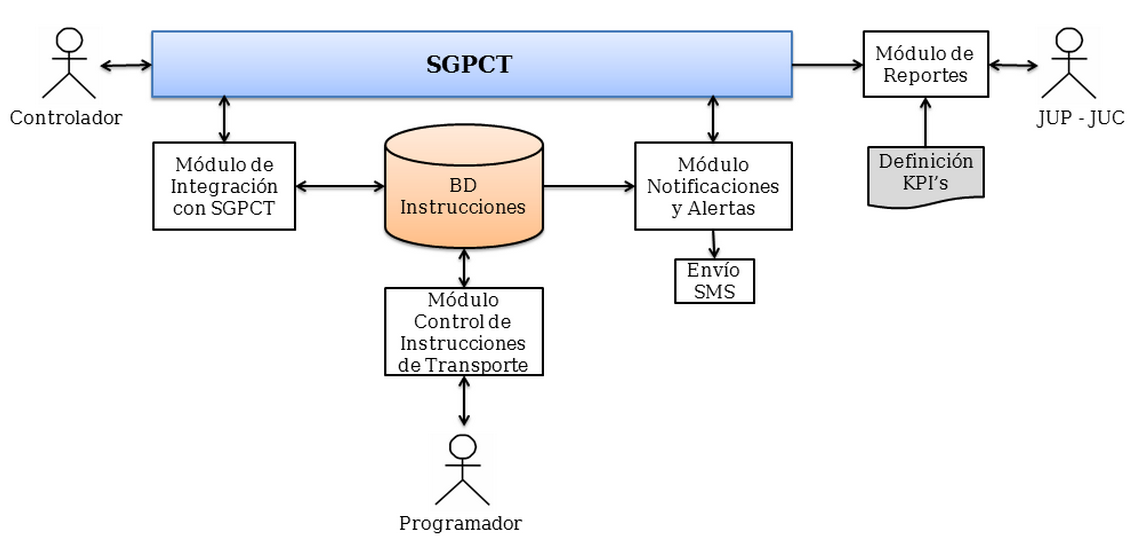
\includegraphics[scale=0.4]{./images/DiagramaPTT}
    \caption{Módulo de Instrucciones y SGPCT}
    \label{fig:diagramaPTT}
\end{figure}

Se explica a continuación el detalle de cada componente mostrado en el diagrama.

\subsection{Módulo de control de instrucciones de transporte}
Permite al asistente de programación y al jefe de la unidad de programación ingresar todas las instrucciones, modificarlas o eliminarlas según corresponda de manera diaria. Las instrucciones generales se ingresan mediante una interfaz gráfica que contiene todas las especificaciones requeridas por una instrucción. Las instrucciones generadas a partir de la programación se formarán automáticamente mediante el cálculo de la diferencia entre la regla base que define el programa y la programación particular del día. Las instrucciones se clasifican de acuerdo a las dimensiones definidas anteriormente.

\subsection{Módulo de notificaciones y alertas}
Se encarga de informar a los controladores y administrativos de manera oportuna sobre las instrucciones que deben realizarse a cada momento y les permite indicar si se han realizado con éxito o no. Contempla el envío de mensajes a los celulares definidos para las jefaturas de la UCT y la UPT.

\subsection{Módulo de integración con SGPCT}
Contempla la relación con el SGPCT de los nuevos módulos asociados a las instrucciones, notificaciones y alertas. Contempla toda la interfaz requerida para la integración adecuada entre los dos sistemas.

\subsection{Módulo de reportes}
Permite obtener reportes a los jefes de unidad de programación y control en base a los indicadores de rendimiento definidos y a los datos generados de la operación diaria. Los reportes generados en este módulo se basan en la definición realizada de los KPI de acuerdo a lo especificado en el documento de especificación de requerimientos.

\subsection{Base de Datos de Instrucciones}
Se integró una nueva base de datos al SGPCT de acuerdo a lo definido en el modelo de datos (se muestra el diagrama del modelo relacional implementado en la figura \ref{fig:BD_INSTRUCCIONES}. Se debe notar que ha sido necesario asociar las tablas ya existentes en las bases de datos del SGPCT con las nuevas tablas requeridas por el módulo de instrucciones. 

Los datos son ingresados a esta base de datos desde el módulo de control de instrucciones de transporte. Las instrucciones almacenadas alimentan el módulo de notificaciones y alertas. El módulo de integración con el SGPCT depende de esta base de datos para su funcionamiento. El módulo de reportes obtendrá los datos necesarios a partir de la información contenida en esta base de datos en particular y las tablas asociadas propias del SGPCT.

\section{Entregables finales}
El prototipo entregado contempló una versión inicial de todos los módulos propuestos en la solución. El nuevo módulo se encuentra integrado con el SGPCT en su ambiente de desarrollo, y se ha considerado fuera del alcance del periodo de práctica el traspaso a producción.

Entre los indicadores implementados en el prototipo entregado se encuentra la DPP. El reporte entrega la desviación por cada tren y la desviación agregada de todos como se definió anteriormente. También, se genera un reporte similar para los tiempos de salida y tiempos de llegada. En la fórmula simplemente se cambian los tiempos de viaje por tiempos de salida y de llegada respectivamente (estos tiempos se toman con respecto al inicio de la jornada). El resultado de este reporte puede visualizarse en el anexo D.

Otro de los indicadores implementados en el prototipo entregado es el NCI. El sistema es capaz de entregar el nivel de cumplimiento de instrucciones de manera diaria. Además, en caso de no reportarse la novedad necesaria los jefes de la UCT y UPT les interesaba conocer los controladores que no cumplían con este paso del procedimiento, esto también ha sido convertido en un reporte. Se pueden ver los dos reportes generados en al anexo D.

\chapter[Levantamiento de Procesos de Maniobras]{LEVANTAMIENTO DE PROCESOS DE MANIOBRAS}
El propósito de este capítulo es explicar el trabajo realizado en el modelamiento y análisis de los procesos de maniobras de trenes de línea.

\section{Descripción de la situación actual y problemática}
La seguridad operacional es una de las principales prioridades dentro del FCAB, y es por ello que existe una constante preocupación de mejorar este factor en el desarrollo de los servicios diarios. Actualmente el DCSO cuenta con varios manuales que describen los procedimientos y protocolos que se deben seguir al momento de realizar maniobras con los trenes (entiéndase como maniobra toda acción que involucre tomar o dejar carros y/o locomotoras). No obstante, no existe forma de verificar que estos procedimientos son acatados y se debe confiar exclusivamente en la palabra de los operadores. Claramente, esta situación no es óptima y da paso a una serie de riesgos durante la operación, y en caso de ocurrir un incidente no se cuenta con ningún respaldo formal de los pasos realizados.

La falta de respaldo formal y de un método de verificación de los procedimientos ha provocado una serie de quiebres en la operación, que en algunos casos han resultado en sanciones menores y en el peor caso han llevado a la muerte de operadores. Todo esto causado por la negligencia de los operadores al no seguir los procedimientos de seguridad preestablecidos. 

Producto de los incidentes anteriores, el DTIC ha propuesto al DCSO la implementación de un sistema que permita verificar la correcta ejecución de las maniobras. Inicialmente se pretende utilizar una checklist que registre la realización de cada paso del proceso en los TVL actualmente instalados en cada locomotora. En el marco de esta propuesta se contempla el levantamiento de los procesos de maniobras de trenes de línea y la formulación de las propuestas iniciales para la posterior realización del proyecto.

\section{Objetivos}
En las reuniones iniciales con el jefe del DTIC y jefe del DCSO se definieron los objetivos que debería cumplir el nuevo sistema. El propósito del proyecto es el desarrollo de un nuevo sistema de apoyo al control de las maniobras. El objetivo general de este nuevo sistema es controlar la correcta ejecución de las maniobras de línea y verificar que se sigan los procedimientos preestablecidos.

Los objetivos específicos que debe cumplir el nuevo sistema son:
\begin{itemize}
\item Registrar el desarrollo de los procedimientos de las maniobras de línea.
\item Minimizar el riesgo de error humano en los procedimientos de maniobras por omisión de pasos.
\item Controlar el cumplimiento de los procedimientos oficiales de maniobras de línea.
\item Integrar el nuevo módulo de maniobras con el SGPCT.
\end{itemize}

\section{Levantamiento de procesos y análisis}
El levantamiento contempló las siguientes actividades:

\begin{itemize}
\item Estudio de manuales de procedimientos oficiales.
\item Estudio de la representación de las maniobras en los sistemas.
\item Observaciones in situ.
\item Desarrollo de modelos preliminares.
\item Reuniones con expertos en seguridad operacional del ferrocarril.
\end{itemize}

La principal actividad realizada fue la observación de los procesos de maniobras en el sector de Mejillones, donde, bajo la supervisión de uno de los encargados de seguridad operacional, se presenciaron todas las actividades requeridas para las maniobras de tomar y dejar carros. El objetivo de estas actividades era familiarizar al equipo de trabajo en la compleja naturaleza de las maniobras ferroviarias. Durante el trayecto de Mejillones al terminal del puerto se tuvo la oportunidad de conversar con los operadores de trenes, de esto se obtuvo información referente al desarrollo de las maniobras y al funcionamiento del TVL dentro de la locomotora.

En base a las observaciones realizadas en terreno, el estudio de los procedimientos oficiales, se detectaron ocho tipos de maniobras diferentes. El objetivo de estas normativas es asegurar que los equipos detenidos no se deslicen, desrielen, escapen o tengan desplazamientos no deseados.

Los tipos de maniobra definidos en la documentación oficial son los siguientes: tomar carros en estación, dejar carros en estación, tomar locomotoras en estación, dejar locomotoras en estación, colocar carros en postura para carguío en terminales, retirar carros cargados de terminales, colocar carros a la descarga en terminales y retirar carros descargados desde terminales. Estos procedimientos se encontraban clasificados y registrados de forma genérica dentro del SGPCT, de acuerdo a una serie de códigos predefinidos.

Estos procedimientos poseen un gran cantidad de variantes y casos específicos que deben ser tratados de manera diferente, debido a esto, el objetivo planteado en esta primera fase de levantamiento fue la construcción de modelos genéricos que permitiesen describir las generalidades de las maniobras. En el anexo C se muestran se presentan los modelos desarrollados para los diferentes procedimientos especificados en los manuales e instructivos.  

\section{Propuesta de solución}
\subsection{Idea general}
La propuesta consiste en la implementación de un nuevo módulo para el TVL existente en cada locomotora, correspondiente a una checklist para cada procedimiento. Esta lista contendrá los principales pasos de cada maniobra, de acuerdo a lo especificado en el manual de operaciones y los instructivos de procedimientos.

Cada vez que se vaya a realizar una maniobra el maquinista deberá escoger en el sistema el tipo de maniobra a realizar y en base a esto se mostrará la serie de pasos a seguir. Durante el desarrollo de la maniobra el operador deberá marcar cada paso que se realiza, si es necesario se anexará datos pertinentes a dicho paso para su posterior uso en el control de las maniobras. 

Actualmente la maniobra se coordina entre los operadores mediante el uso de radio en canal local, esta lógica de operación se mantendrá, pero se incorporará que el maquinista ingresará la información en el sistema a medida que su ayudante se la comunique. Cada tipo de maniobra tendrá asociada una secuencia de pasos que deben ser verificados de esta forma. La ejecución de cada maniobra quedará registrada en conjunto con el tiempo en que se realizó cada paso y los datos que correspondan, esta información será utilizada en el posterior control de los procedimientos por parte de los supervisores.

Por otra parte, el sistema deberá ser implementado de tal forma que sea simple realizar cambios en los flujos de trabajo, para ello se contempla el uso de un lenguaje de modelado de procesos o workflows que permita mantener eficientemente la base de conocimientos que contiene los modelos.

\subsection{Plan piloto}
Dado el nivel de complejidad descubierto en el desarrollo de maniobras. En conjunto con los encargados de seguridad operacional se propuso un plan piloto para el desarrollo del proyecto. La propuesta consiste en realizar un análisis detallado de los procedimientos de maniobras para un tren crítico, con su posterior implementación en el TVL. Esto con el objetivo de evaluar la factibilidad y aporte real entregado por el proyecto.

Los modelos desarrollados en el levantamiento inicial presentan el esquema general de las maniobras, no obstante, debido a la complejidad y multitud de casos que pueden darse en la operación real de los trenes, se hace imposible mostrar todos los detalles del proceso en un solo modelo. El esquema general presentado deberá ser adaptado para cubrir las particularidades de cada tren en cada terminal que corresponda.

Se utilizará una lista de trenes críticos definidos por la jefatura de la UCT, quien debería indicar que trenes presentan la mayor cantidad de conflictos a nivel de desarrollo de maniobras. En base a esto se determinaría en qué tren se debe implementar el plan piloto.

Una vez construido el modelo detallado para el primer tren se implementaría el prototipo del nuevo sistema para evaluar su funcionamiento y determinar si el proyecto debe continuar. En caso ser exitoso el plan piloto, se deberá iniciar el análisis de los procesos para cada uno de los trenes restantes, este proceso debe ser exhaustivo y detallado. Es necesario estudiar las variaciones de los procesos para cada tren y en cada estación, no se pueden omitir estos pasos en los modelos pues cada paso es vital para la seguridad de la operación. 

\subsection{Integración con SGPCT}
El SGPCT actualmente almacena como caja negra los procesos de las maniobras, indicando simplemente que el tren se encuentra realizando una. Interesa que durante los estados en que el tren se esté realizando una maniobra el módulo del TVL se mantenga sincronizado con la información del SGPCT.

El SGPCT tendrá ingresada la información del inicio y término de la maniobra, mientras que el nuevo sistema entregaría el detalle interno de las maniobras de acuerdo a los modelos de procesos definidos. Esta información podría ser utilizada por control con el fin de saber el estado de una maniobra, permitiéndole a los controladores de trenes manejar de mejor forma el flujo ferroviario.

\subsection{Análisis de tiempos de proceso y conformidad}
Uno de los beneficios colaterales obtenidos con el desarrollo de este proyecto es que será posible realizar análisis más detallado de los tiempos de maniobra, pues se tendrá información completa del desarrollo a nivel operacional. Además permitiría detectar anomalías y tiempos inusuales de proceso.

Por otro lado, mediante el uso de los datos almacenados en el sistema y la definición de los diferentes modelos, sería posible implementar un algoritmo que revise la conformidad de los eventos reales con la definición de los workflows originales.

Los algoritmos permitirán determinar las discrepancias entre el modelo definido y la operación real en base a los tiempos de cumplimiento que indique los operadores. Incluso, se podría utilizar esta herramienta para medir las desviaciones anómalas en los tiempos de ejecución de las maniobras. La complejidad asociada a esta propuesta es el uso de algoritmos y herramientas avanzadas de minería de procesos (Van Der Aalst, 2011).

\chapter[Otras Actividades]{OTRAS ACTIVIDADES}
Se presentan a continuación una serie de trabajos realizados durante el periodo de práctica, que no caen directamente dentro del marco de los dos proyectos principales asignados.

\section{Requerimientos ingenieros de servicios}
Una de los trabajos que debió ser atendido durante el periodo de práctica corresponde al levantamiento de requerimientos del área de servicios del FCAB. Este trabajo consideró dos reuniones con los ingenieros de servicios con el fin de capturar sus inquietudes y necesidades, además de entender sus funciones dentro de la empresa. Además, fue necesario realizar un análisis de las planillas y la forma de trabajo actual.

Actualmente el proceso de control de cumplimiento de tonelaje se realiza mediante planillas electrónicas diferentes definidas por cada ingeniero de servicio en función de las necesidades de cada servicio que atiende. La información que contienen es similar, pero no existe un formato estándar en estas.

Los valores numéricos asociados al tonelaje se obtienen del sistema revisando manualmente de forma diaria. Esta parte del proceso es muy sensible a error humano, la idea es que estos datos se rellenen de forma automática desde el sistema, sin que los ingenieros tengan que invertir tiempo obteniéndolos.

En caso de no cumplirse el programa (el nivel de cumplimiento esperado debe ser sobre 90\%) se debe justificar los motivos, actualmente esta parte se debe realizar de forma manual a partir del registro de novedades diario. Debido a que los reportes de novedades no siempre contienen información completa se hace necesario realizar un proceso de rastreo de causas e inferencia. Esta parte no se considera factible automatizar totalmente, debido a que el proceso de inferencia es particularmente complejo, en el mejor caso se podría utilizar la clasificación de novedades actual para explicar estas causas.

Se contempla también la necesidad de que la información se encuentre disponible oportunamente en tiempo real, pues actualmente existe un desfase notorio entre la ocurrencia de los quiebres y el reporte correspondiente al ingeniero de servicio. Esto se realizaría mediante el uso de notificaciones y de indicadores. La principal causa de la falta de información oportuna se debe a que durante el ciclo de vida del tren existen etapas que no son visibles fácilmente, y por lo tanto se dificulta llevar un control adecuado de ellas.

El levantamiento de requerimientos y la propuesta inicial fue entregada en un documento formal a los ingenieros de servicio y al encargado de práctica. En base a las propuestas realizadas se pretende realizar un proyecto que contemple la profundización, desarrollo e implementación de éstas. No obstante, debido a la falta de personal disponible y la baja prioridad de los requerimientos se ha postergado el proyecto hasta tener mayores recursos humanos disponibles.

La propuesta tiene por objetivo implementar una mejora en el SGPCT que permita llevar un seguimiento a la programación y ejecución, con el fin de detectar las causas de los incumplimientos en los niveles de servicio. 

Los objetivos específicos son:
\begin{itemize}
\item Automatizar el proceso de control de los servicios con respecto al cumplimiento de tonelaje.
\item Cuantificar las pérdidas asociadas a los servicios con respecto a las causas correspondientes.
\item Evidenciar las causas raíces de los incumplimientos de los servicios por atender.
\item Eliminar los vacíos de información en el ciclo de vida del tren.
\end{itemize}

consiste en empezar por la automatización del traspaso de datos manual desde el sistema a las planillas, esto debido a que actualmente la etapa del proceso más propensa a error humano. La parte de búsqueda de causas raíz se podría complementar utilizando la clasificación de las novedades, aunque para causas más complejas será necesario que el usuario analice manualmente las posibilidades. Será necesario hacer un análisis de los posibles tipos de causas.

Se determinó que será necesario realizar un análisis completo del ciclo de vida del tren, esto con el fin de generar un modelo detallado que identifique dónde se encuentran los vacíos de información. Una vez realizado este análisis sería necesario definir qué eventos del ciclo de vida del tren y novedades correspondientes es necesario notificar a los ingenieros de servicio con el fin de minimizar los incumplimientos.

El sistema propuesto utilizaría la información del tonelaje perdido por cada causa con el fin de proporcionar información en forma de un reporte detallado o mediante un dashboard. Esto implicará redefinir la forma de identificar las variables que influyen en la operación de los servicios, mostrando y cuantificando su participación en el incumplimiento.


\section{Planilla KPI de mantención}
El segundo de los trabajos menores que debió ser atendido durante el periodo de práctica corresponde a la construcción de una planilla de cálculo para un KPI de la Gerencia Mantención Material Rodante e Infraestructura Ferroviaria (GMMRIF), y su posterior validación. Este trabajo consideró el desarrollo y construcción de una planilla en base a las fórmulas preestablecidas y los datos entregados por la GMMRIF.

La razón por la cuál se solicitó la construcción de esta planilla era validar el cálculo realizado por el sistema de mantenciones. Debido a una falla en la definición de la consulta a la base de datos en el sistema, la GMMRIF se encontraba operando con valores incorrectos de un indicador crítico referente a la cantidad de locomotoras en mantención en un instante cualquiera. El quiebre detectado requirió el desarrollo de esta planilla que permitiese calcular el indicador en base a las definiciones iniciales con el fin de poder regenerar la consulta de manera adecuada y sin fallas. 

El quiebre producido por esta falla en el cálculo del KPI fue tan grave para la GMMRIF que fue un factor importante en el despido del encargado del sistema, producto de reiterados problemas y las repercusiones de la esta última falla.

\section{Análisis para actualización remota de TVL}
El tercero y último de los trabajos menores que debió ser atendido durante el periodo de práctica corresponde al análisis del algoritmo rsync para la actualización remota de los TVL. Debido a que al momento de realizarse esta solicitud de trabajo quedaba una semana para finalizar el periodo de práctica, solo se alcanzó a realizar una breve investigación que delineó las bases del futuro trabajo a realizar durante el periodo de marzo fuera de la práctica. 

La motivación tras el análisis de este algoritmo es que las velocidades de transferencia a un TVL son demasiado bajas y las conexiones particularmente inestables debido a los recorridos de los trenes, que actualmente para realizar una actualización a los dispositivos es necesario ir de forma presencial a cada tren y realizar la actualización, pues cualquier intento de actualización remota es demasiado lento.

Para poner en perspectiva la lentitud de la conexión, como referencia se entrega que una transferencia de 500 kilobytes requeriría de alrededor de 30 minutos, considerando la cantidad de locomotoras que tiene el FCAB y que actualmente los archivos a transferir pesan aproximadamente 10 megabytes, es claramente poco práctico utilizar un método de actualización remota que requiera el traspaso del archivo completo.

Es por ello que se solicitó la búsqueda de una herramienta que permitiera actualizar de forma remota y rápida los TVL. La investigación inicial permitió dar con el algoritmo rsync para la actualización remota. Este algoritmo utiliza una estrategia que permite detectar las diferencias reales entre los archivos antiguos a actualizar y las nuevas versiones, permitiendo ahorrar ancho de banda y tiempo de transferencia, siendo diseñado inicialmente para conexiones inestables y lentas como las del TVL.

La investigación requirió la lectura y análisis del artículo original que describe rsync y además la búsqueda de alternativas de solución. Entre lo primero que se intentó, fue buscar herramientas preexistentes que implementar este tipo de actualización. El principal problema enfrentado es que el sistema operativo utilizado por los TVL (Windows CE) no poseía ninguna implementación del algoritmo rsync o alguna herramienta similar, tanto nativa como de un desarrollador independiente, por lo que sería necesario realizar un desarrollo propio del algoritmo. Este desarrollo por supuesto quedó fuera del alcance del periodo de práctica.

\chapter[Conclusiones]{CONCLUSIONES}
Si bien la informática es solo una actividad de apoyo dentro de la cadena de valor para el FCAB, su importancia se puede ver en todas las actividades desarrolladas durante este periodo de práctica. El trabajo realizado por el DTIC se ha vuelto crucial dentro de la operación de la empresa, en este contexto, la mejora continua de los sistemas actuales y sus procesos es de vital importancia para mejorar la calidad del servicio entregado.

En el aspecto de programación y control de los trenes, la mejora de estos procesos y del SGPCT permitió apoyar la operación diaria del ferrocarril y además facilitar el trabajo del DPCT, área que actualmente posee una gran carga laboral y altos niveles de estrés, que a la larga repercuten en la productividad. 

Por otro lado, en el marco de la seguridad operacional, el modelamiento de los procesos de maniobras y la subsecuente propuesta realizada permitirá al DTIC apoyar al DCSO en este proyecto conjunto para controlar los procesos de maniobra, repercutiendo así sobre la operación del ferrocarril y mejorando los indicadores de seguridad.

Debido a que la práctica fue concebida inicialmente bajo la idea de realizar análisis y diseño de soluciones, la implementación completa de éstas se ha considerado fuera del alcance del periodo de práctica. No obstante, las actividad realizadas han sentado las bases para futuros proyectos del DTIC en conjunto con otros departamentos, tales como el DCSO, el DPCT y el área de servicios.

El trabajo contemplado a futuro después de la finalización del periodo de práctica es el desarrollo del sistema completo para el programa de transporte de trenes, saliendo ya del marco de los prototipos, y traspasando el módulo de instrucciones a producción. En lo referente al modelamiento de maniobras, este trabajo ha sido finalizado en su etapa inicial de levantamiento, y el proyecto será abordado por otros ingenieros dentro del DTIC. 

En cuanto a los otros trabajos realizados, para los requerimientos de los ingenieros de servicio no se han contemplado proyecciones futuras de trabajo, principalmente porque se ha solicitado continuar con el trabajo en el algoritmo rsync.

La mayor dificultad encontrada durante el desarrollo de la práctica fue la falta de claridad de los stakeholders en los requerimientos del módulo de instrucciones para el programa de transporte de trenes, este es un problema común dentro de la ingeniería de requisitos y existen una serie de técnicas para clarificar los requerimientos, entre ellas el desarrollo de prototipos (Sommerville, 2011), que fue justamente el enfoque utilizado para clarificar las ambigüedades.

A nivel personal, esta segunda práctica ha servido como una buena experiencia laboral y ha sido de gran ayuda para crecer como profesional. A diferencia de la primera práctica que puso a prueba competencias más técnicas referente al desarrollo de software, ésta se centró más en competencias blandas tales como las capacidades comunicativas, la adaptabilidad y el trabajo colaborativo.  Principalmente debido al hecho que una gran parte de la práctica correspondió al levantamiento de requerimientos y procesos, lo que implicaba un alto nivel de interacción con los clientes y usuarios, además de cambios constantes en los requisitos.

También se vieron empleadas habilidades tales como la capacidad de organización, debido a la alta carga impuesta por los múltiples trabajos abordados, fue necesario realizar una planificación detallada de las actividades a realizar, y el autoaprendizaje, debido a que en muchos casos no se pudo contar con apoyo directo, debido a la carga laboral de los ingenieros del DTIC, y fue necesario investigar el funcionamiento de las diferentes herramientas.

Además, también ha sido un aporte el tener la oportunidad de enfrentar un ambiente laboral nuevo, en el que ha sido necesario no solo interactuar con otros ingenieros en la búsqueda de soluciones, sino que gracias a la naturaleza del trabajo se ha conocido incluso el nivel operacional de la empresa, lo que ha permitido enriquecer la formación necesaria para un Ingeniero Civil en Computación e Informática antes de salir al mundo laboral.

En general la formación entregada por la universidad, en particular la capacidad de autoaprendizaje y el trabajo en equipo, fueron vitales para el desarrollo de la práctica. Se pudo utilizar gran cantidad de los conocimientos adquiridos durante la carrera, con especial énfasis en lo que corresponde al levantamiento de requerimientos,  modelamiento de procesos, análisis, y gestión de proyectos.

Finalmente, dados los puntos anteriores, se afirma que el desarrollo de esta práctica ha sido beneficioso tanto a nivel personal como para la empresa. Se han cumplido todos los objetivos planteados por el FCAB en los dos proyectos abordados, y además los propios correspondientes a la segunda práctica pre profesional, al haber utilizado los conocimientos y destrezas adquiridas en el transcurso de la carrera en una empresa real.

\renewcommand\bibname{BIBLIOGRAFÍA}
\bibliographystyle{plain}

\def\bibindent{1cm}
\begin{thebibliography}{99\kern\bibindent}%Si tienes más de 99 editar este número a la cantidad de referencias que tengas.
\makeatletter
\let\old@biblabel\@biblabel
\def\@biblabel#1{{}\kern\bibindent} %En el { } agregar \old@biblabel{#1}
\let\old@bibitem\bibitem
\def\bibitem#1{\old@bibitem{#1}\leavevmode\kern-\bibindent\kern-2.1em}
\makeatother

\bibitem{2} Kuhn, T. (2013). Controlled Natural Language and
Opportunities for Standardization. ETH Zurich, Switzerland.

\bibitem{3} Laudon, K. C. y Laudon, J. (2004). Management information systems: managing the digital firm. New Jersey, 8.

\bibitem{4} Louden, K. C. (1997) Compiler Construction: Principles and Practice. PWS Publishing.

\bibitem{5} Porter, M. y Millar, V. (1985). How information gives you competitive advantage. Harvard Business Review: 149 – 160.

\bibitem{6} Schittenhelm, B. y Landex, A. (2012). Danish Key Performance Indicators for Railway Timetables.

\bibitem{7} Sommerville, I. (2011). Software Engineering (9na edición). Boston, USA: Addison-Wesley.

\bibitem{8} Tridgell, A. y Mackerras, P. (1996). The rsync algorithm.

\bibitem{9} Van Der Aalst, W. (2011). Process mining: discovery, conformance and enhancement of business processes. Springer Science \& Business Media.




\end{thebibliography}

\addcontentsline{toc}{chapter}{Bibliografía}


%\mainmatter %Esto hace que los anexos SI tengan numeros de cap.
%Se utilizan letras en vez de numeros.
\titleformat{\chapter}[hang]
{\fontsize{12}{12}\bfseries}
{ANEXO\hsp\Alph{chapter}{.}\hsp}{0pt}{\fontsize{12}{12}\bfseries}
\titlespacing{\chapter}{0cm}{-13.6pt}{0.21cm}[0cm]

%Se utilizan letras en vez de numeros.
\renewcommand{\thesection}{\Alph{chapter}.\arabic{section}}
\renewcommand{\thefigure}{\Alph{chapter}.\arabic{figure}}
\renewcommand{\thetable}{\Alph{chapter}.\arabic{table}}

%Se inician los apendices.
\begin{appendices}
\renewcommand\appendixname{Anexo}

\chapter[Planificación]{PLANIFICACIÓN}
\begin{figure}[H]
\centering
    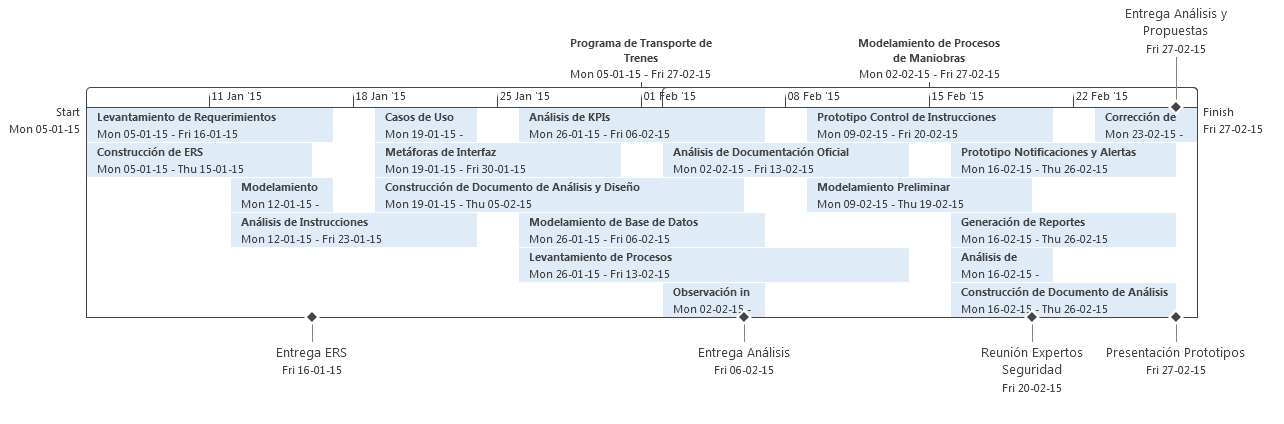
\includegraphics[angle=90,scale=0.60]{./images/Gantt}
    \caption{Carta Gantt simplificada}
    \label{fig:Gantt}
\end{figure}

\chapter[Gramática para Instrucciones]{GRAMÁTICA PARA INSTRUCCIONES}
{\setstretch{1.0}
\begin{enumerate}
\item instruccion ::= lista\_maniobras (val\_requerida \textbf{punto})? | \textbf{excepcion}
\item lista\_maniobras ::= (maniobra \textbf{punto\_coma})* maniobra \textbf{punto}
\item val\_requerida ::= \textbf{validar\_juc} tiempo
\item maniobra ::= (\textbf{negacion})? maniobra\_concreta (val\_requerida)? (\textbf{justificacion} maniobra\_concreta)? (\textbf{coma} restriccion\_global)? 
\item restriccion\_global ::=  \textbf{siempre\_cuando} \textbf{razon\_restriccion}
\item maniobra\_concreta ::=  man\_condicional | man\_agenda | man\_evento
\item man\_condicional ::= \textbf{si} maniobra \textbf{entonces} maniobra (\textbf{otro\_modo} maniobra)? | \textbf{cuando} maniobra \textbf{entonces} maniobra | \textbf{confirmar} \textbf{si} maniobra \textbf{otro\_modo} maniobra
\item man\_agenda ::= \textbf{guion} lista\_objeto \textbf{verbo} (lista\_adjetivo)? (lista\_tiempo)? (lista\_lugar)? | \textbf{verbo} lista\_objeto (lista\_adjetivo)? (lista\_tiempo)? (lista\_lugar)? | interaccion (\textbf{guion} lista\_objeto)? (lista\_tiempo)? (lista\_lugar)?
\item interaccion ::= lista\_objeto (lista\_adjetivo)? \textbf{verbo} lista\_objeto (lista\_adjetivo)? 
\item lista\_objeto ::= (objeto \textbf{guion})* objeto
\item lista\_adjetivo ::= (\textbf{adjetivo} \textbf{guion})* \textbf{adjetivo}
\item lista\_tiempo ::= (tiempo \textbf{guion})* tiempo
\item lista\_lugar ::= (\textbf{terminal} \textbf{guion})* \textbf{terminal}
\item lista\_numero ::= (\textbf{num} \textbf{guion})* \textbf{num}
\item tiempo ::= (\textbf{mod\_tiempo})? (\textbf{hora} (\textbf{posesivo} \textbf{fecha})? | \textbf{fecha}) 
\item objeto ::= (num)? (\textbf{recurso} | \textbf{acc\_recurso} | \textbf{otr\_recurso} | \textbf{personal}) | \textbf{enlace} lista\_numero \textbf{guion} \textbf{terminal} | \textbf{tren} lista\_numero (\textbf{fecha})? | \textbf{loco} lista\_numero | \textbf{vagon} lista\_numero | \textbf{auto} lista\_numero | (\textbf{tratamiento})? \textbf{nombre\_persona} (\textbf{cargo\_persona})? | \textbf{terminal}
\item man\_evento ::= man\_corte\_comunicaciones | man\_mantencion
\item man\_corte\_comunicaciones ::= \textbf{corte\_comunicaciones} lista\_tiempo (\textbf{trabajo} tiempo)? ((\textbf{negacion})? \textbf{apoyo} \textbf{terminal})?
\item man\_mantencion ::= \textbf{mantencion} lista\_objeto lista\_tiempo (\textbf{coma} \textbf{mod\_tiempo} maniobra\_concreta)? \textbf{coma} \textbf{resp\_mantencion} \textbf{nombre\_persona}

\end{enumerate}
}

\chapter[Modelos y Diagramas]{MODELOS Y DIAGRAMAS}

\section{Programa de transporte de trenes}
\begin{figure}[H]
    \centering
    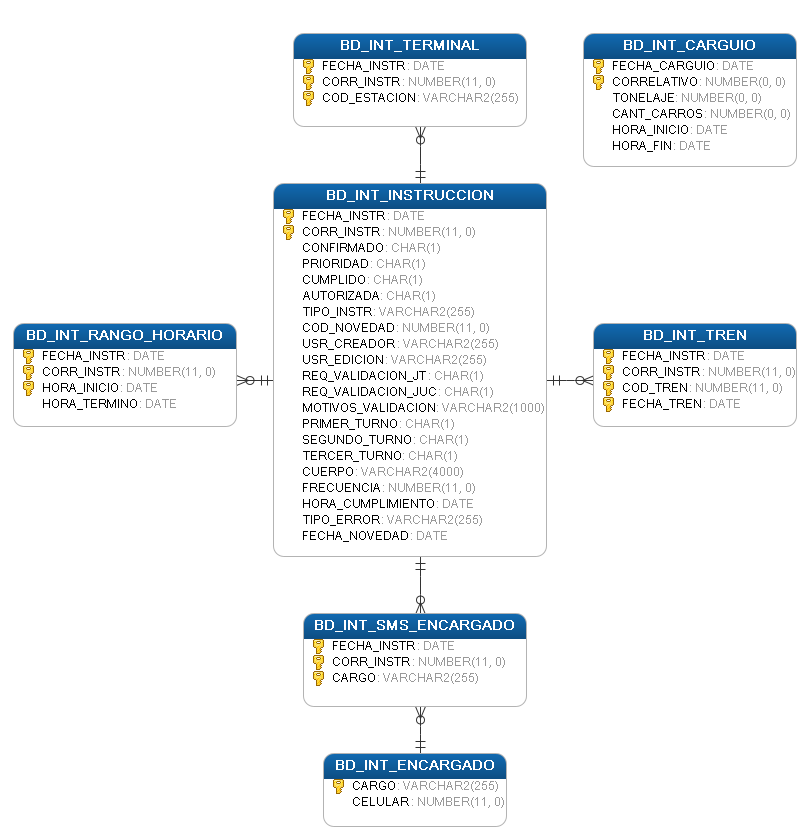
\includegraphics[scale=0.6]{./images/BD_INSTRUCCIONES}
    \caption{Modelo Relacional de la Base de Datos del Módulo de Instrucciones}
    \label{fig:BD_INSTRUCCIONES}
\end{figure}

\begin{figure}[H]
    \centering
    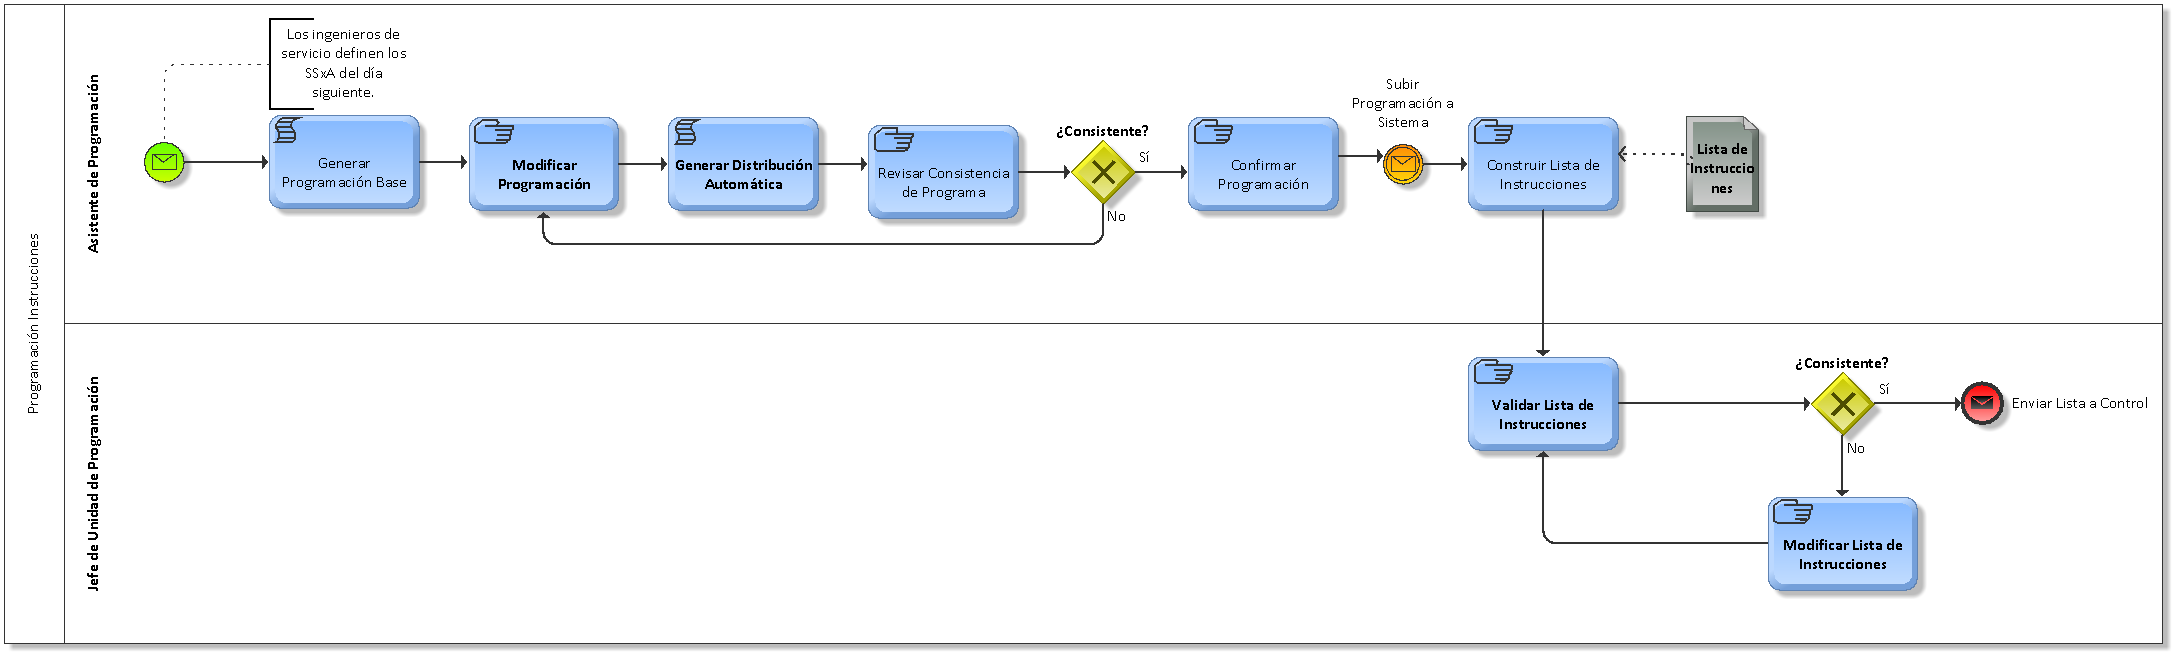
\includegraphics[scale=0.3]{./images/Modelo_Generar_Programacion}
    \caption{Proceso de Programación}
    \label{fig:MGP}
\end{figure}

\begin{figure}[H]
    \centering
    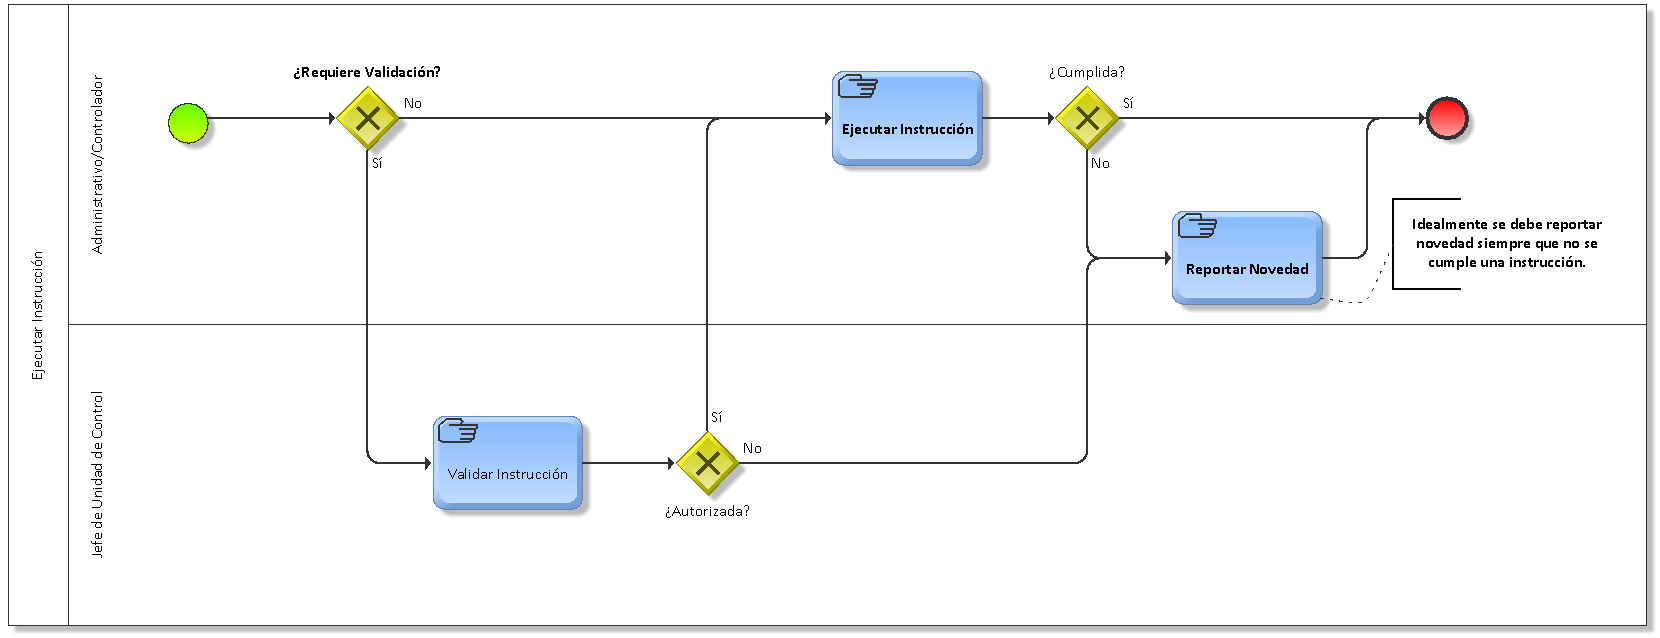
\includegraphics[scale=0.4]{./images/Modelo_Ejecutar_Instruccion}
    \caption{Proceso de Ejecución de Instrucciones}
    \label{fig:MEI}
\end{figure}

\newpage
\section{Procesos de maniobras}
\begin{figure}[H]
    \centering
    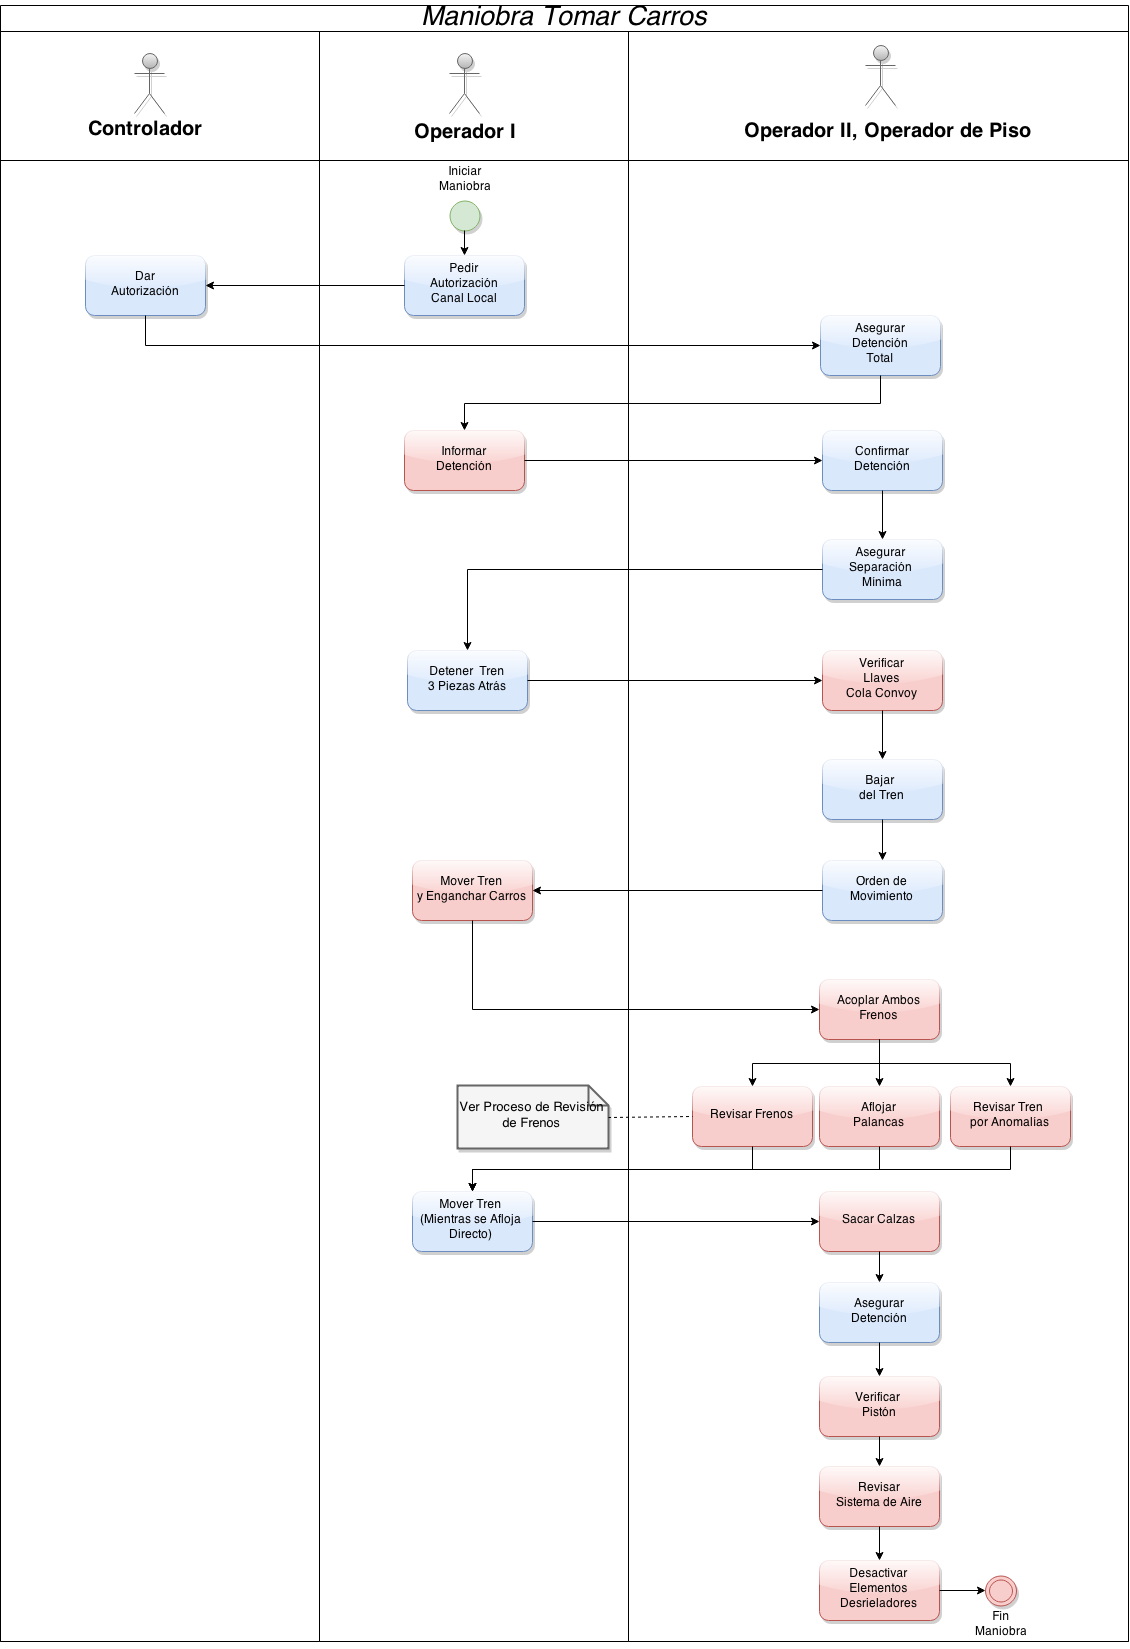
\includegraphics[scale=0.35]{./images/MTC}
    \caption{Procedimiento para Tomar Carros}
    \label{fig:MTC}
\end{figure}

\begin{figure}[H]
    \centering
    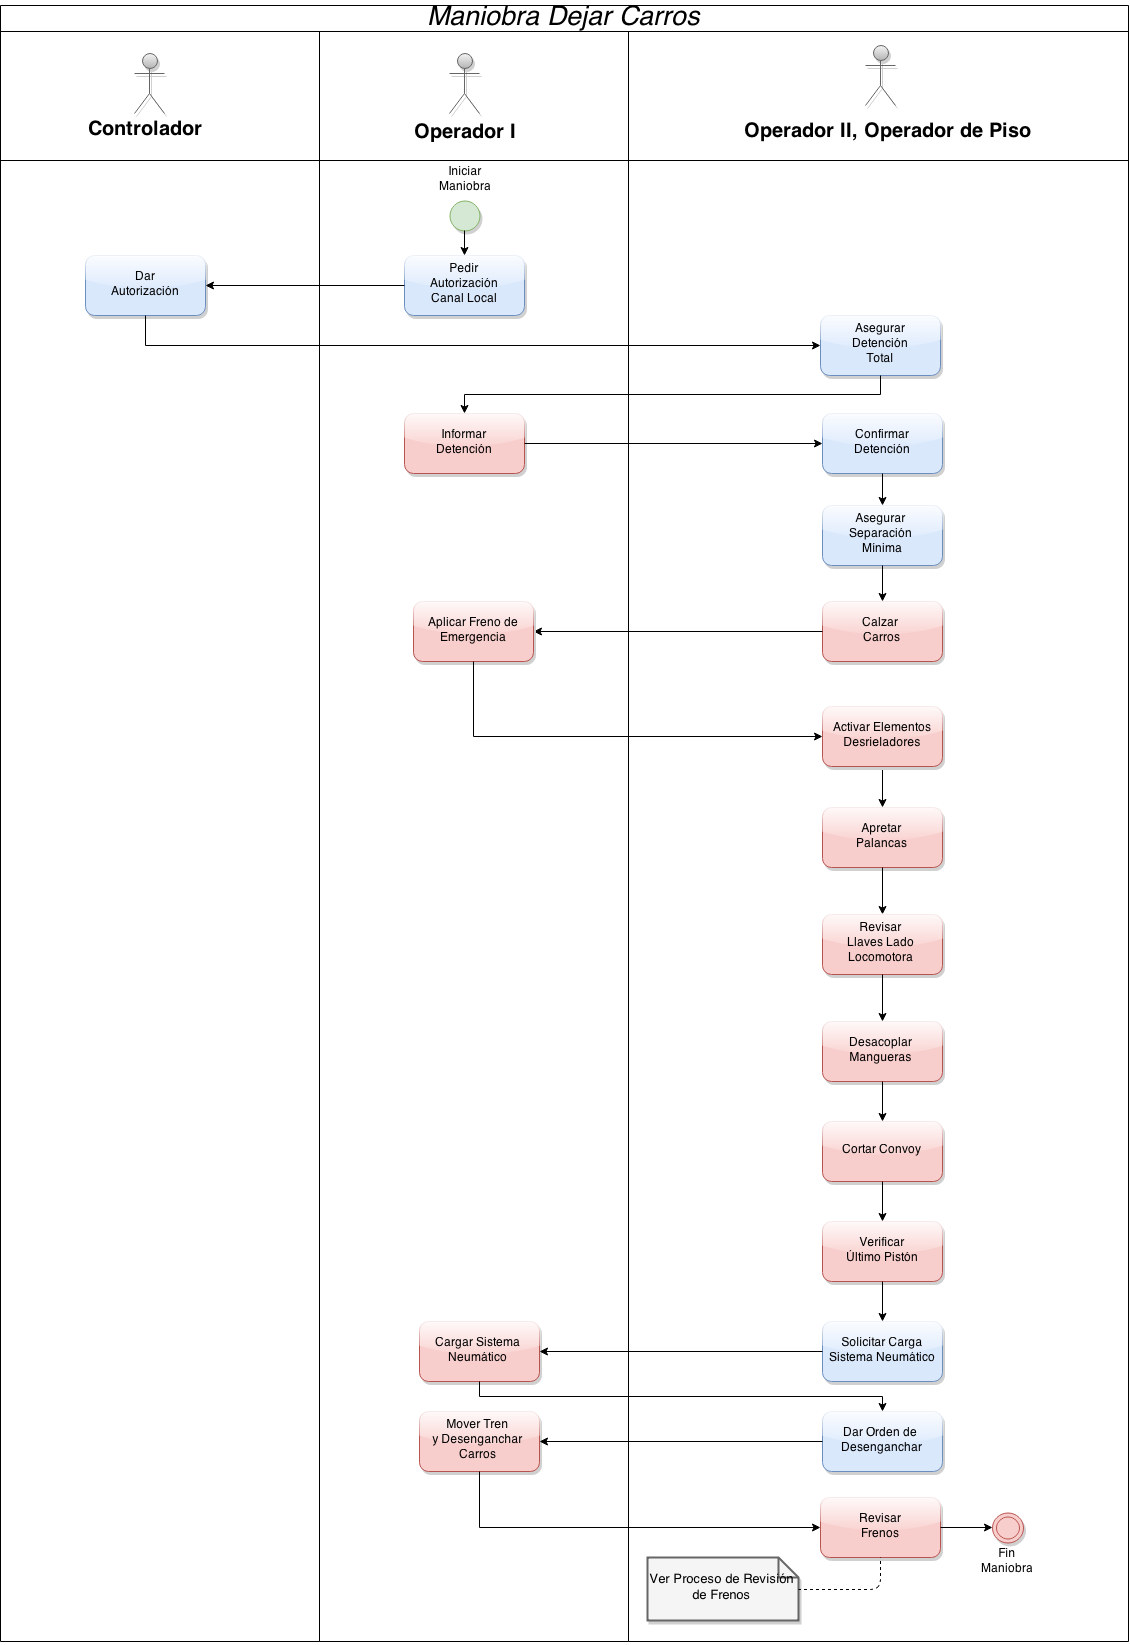
\includegraphics[scale=0.35]{./images/MDC}
    \caption{Procedimiento para Dejar Carros}
    \label{fig:MDC}
\end{figure}

\begin{figure}[H]
    \centering
    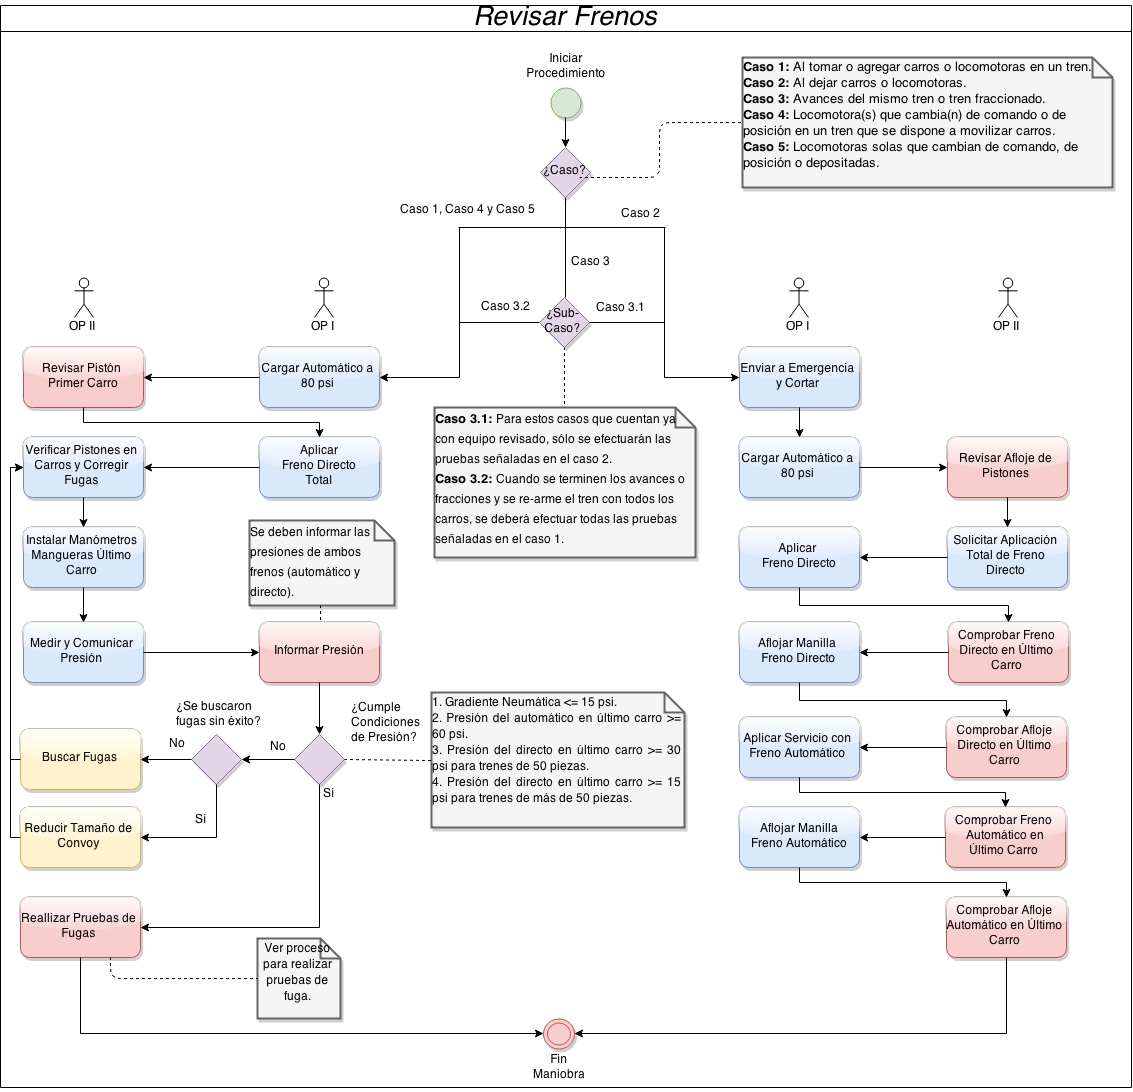
\includegraphics[scale=0.4]{./images/MRF}
    \caption{Procedimiento para Revisar Frenos}
    \label{fig:MRF}
\end{figure}

\begin{figure}[H]
    \centering
    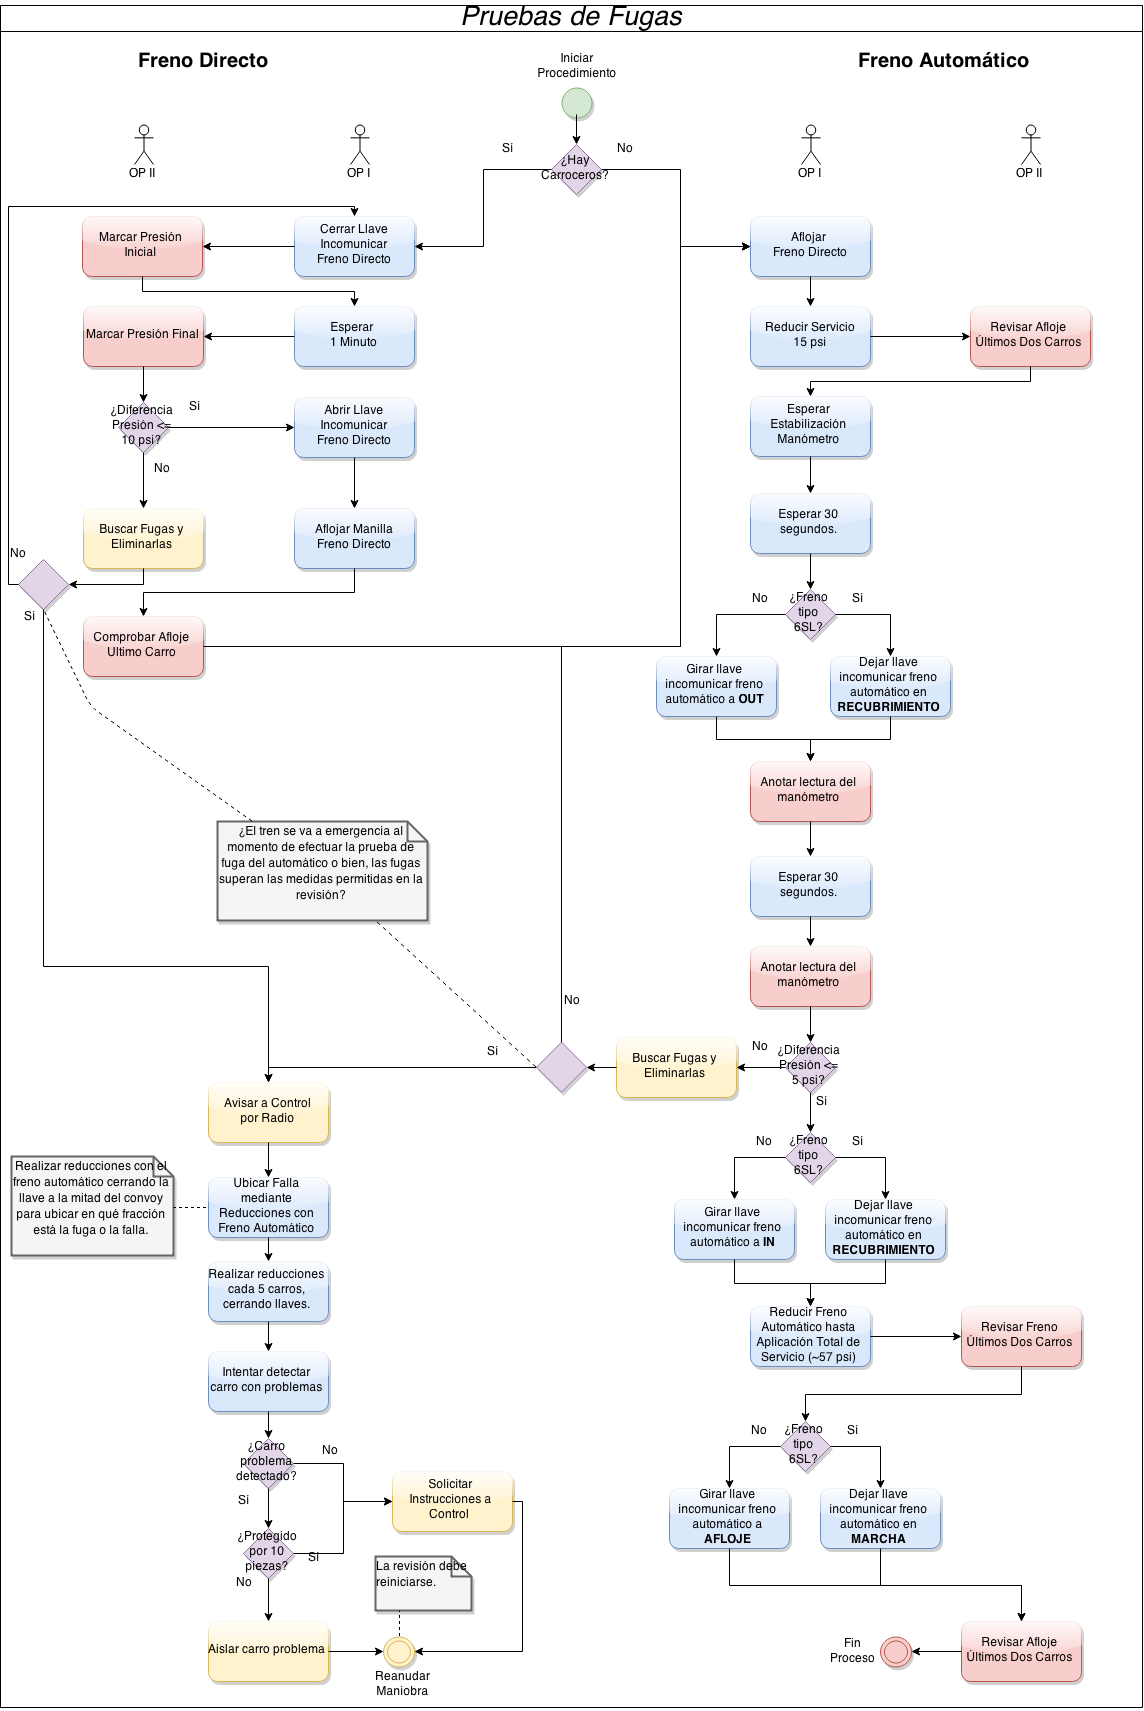
\includegraphics[scale=0.35]{./images/MPF}
    \caption{Procedimiento para Buscar Fallas}
    \label{fig:MPF}
\end{figure}


\chapter[Reportes]{REPORTES}
\begin{figure}[H]
    \centering
    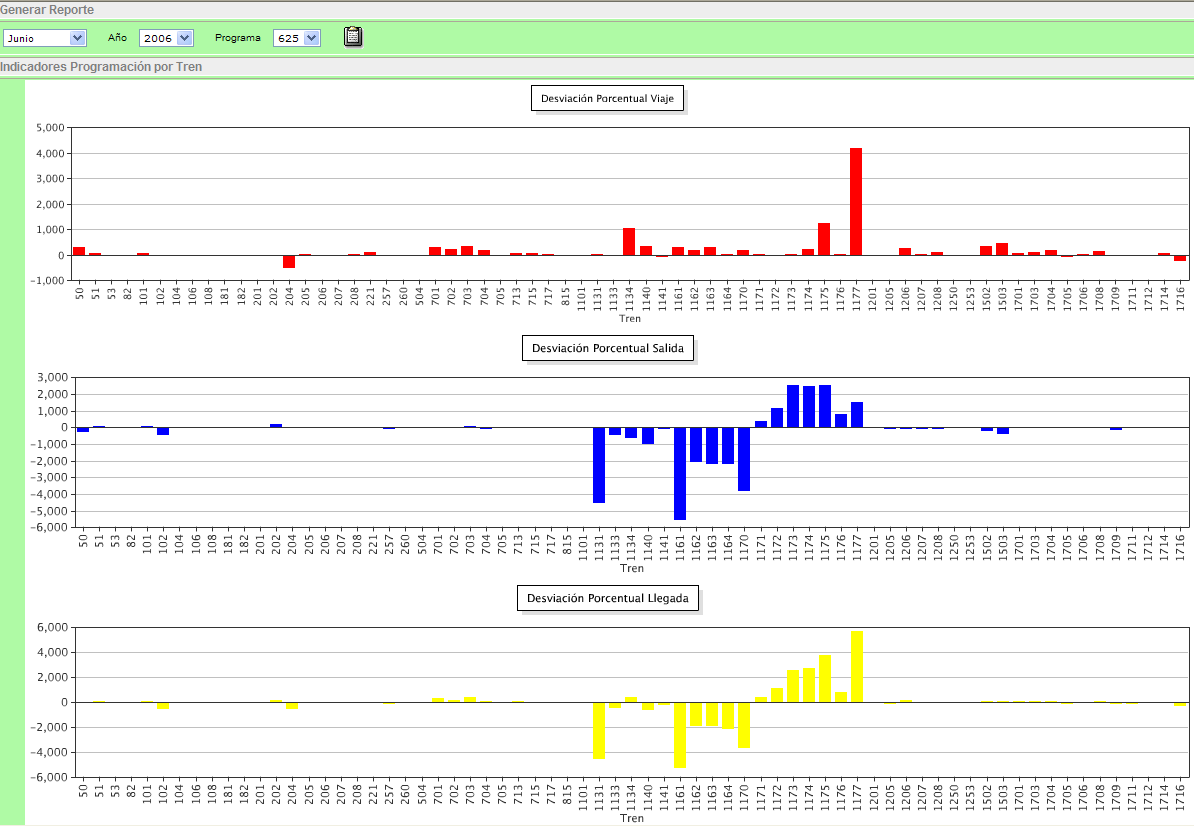
\includegraphics[scale=0.35]{./images/ReporteDesviacionKPI}
    \caption{Reporte de Desviación Porcentual Promedio}
    \label{fig:DPPKPI}
\end{figure}

\begin{figure}[H]
    \centering
    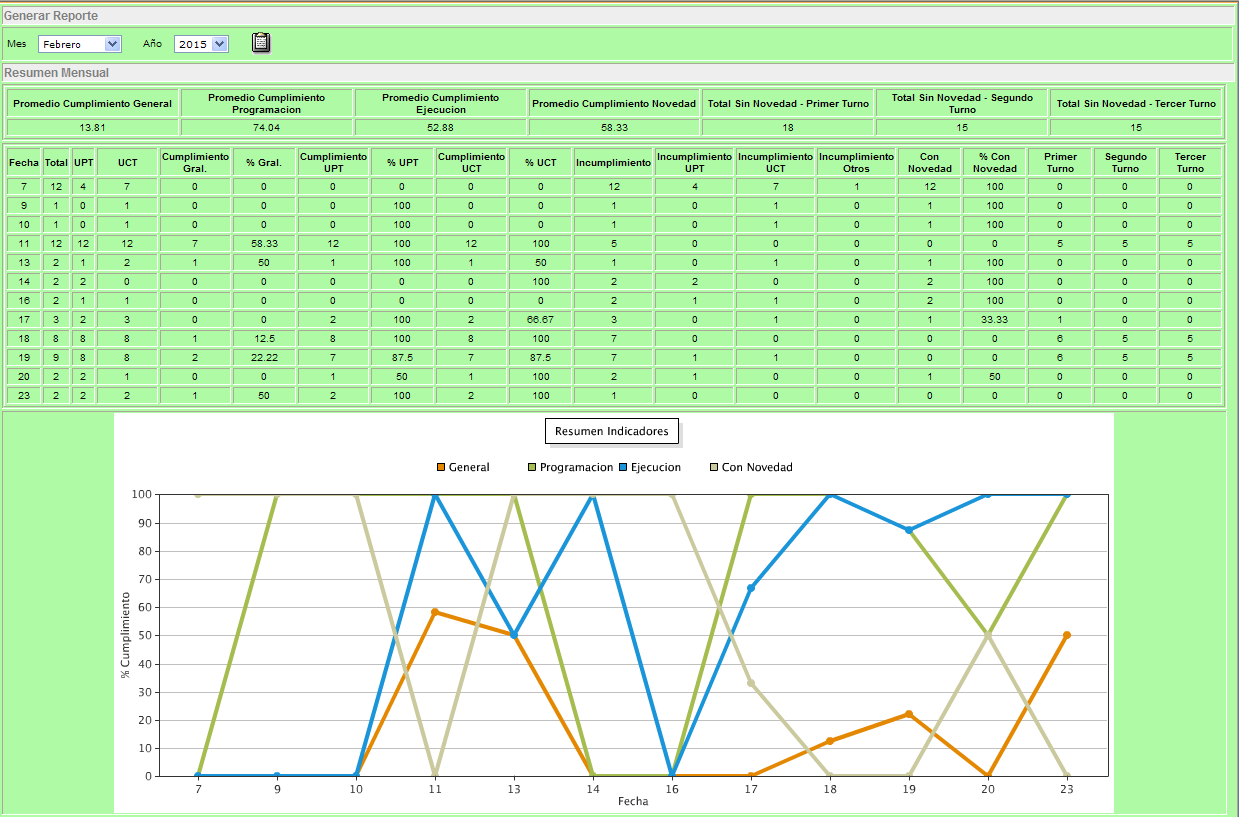
\includegraphics[scale=0.35]{./images/ReporteInstruccionesKPI}
    \caption{Reporte de Cumplimiento de Instrucciones}
    \label{fig:RIKPI}
\end{figure}

\begin{figure}[H]
    \centering
    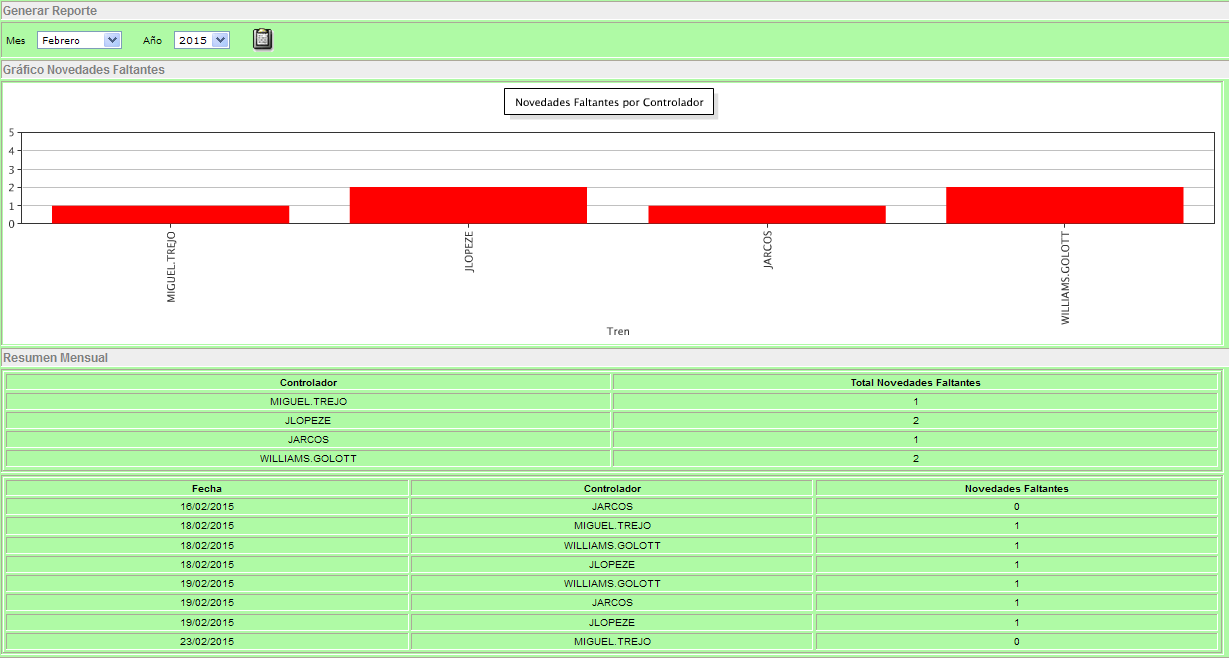
\includegraphics[scale=0.35]{./images/ReporteControladores}
    \caption{Reporte de No Cumplimientos sin Novedad}
    \label{fig:RCKPI}
\end{figure}

\end{appendices}
%--------------------------------------------------------------------------
\end{document}